\label{ca:results}
The results from measurements at DEIF is analyzed to examine if the controller designed in \chapref{ca:controller} is improving the stability of the genset. 

In the generator room located at DEIF four different tests is conducted and the journals in \secref{app:Frequency_steps}, \secref{app:load_steps}, \secref{app:combined_genset_and_inverter} and \secref{app:controller_test} reveals the results of these tests.
The purpose of the first test is to collect data on how a step in frequency affects a real genset at different load sizes, for which to compare with the genset simulink model and the estimated second order model. These tests are named test2-7 as data in test1 was discarded.
The second test is reference measurements of the genset and is named test8-9, the purpose of which to have a base line to compare with at different load steps.
As to get real measurements of the inverter and the genset the third test named test10 were conducted. Problems arose with the inverter which limited the amount of data acquired to a single test, and made the possibility to test the genset with controller in combination with the inverter impossible at the given time.
The fourth test is performed with different scaling factors \ref{system_design_implementation} applied to the designed controller and added to the genset. These tests is named test11-15, and the purpose is to test for any improvement or decrease in stability obtained by the controller designed in \chapref{ca:controller}.

%have been written. The purpose of the first test was to see how the genset reacted to frequency steps with various load shown in \secref{app:Frequency_steps}. These test have been index with test 2 to test 7. The second test was conducted to get some base measurement that could be used to compare the controller up against and is shown in \secref{app:load_steps}. These test are index with test 8 to test 9. The third test was carried out with the inverter and genset sharing the load, to see how the genset reacted when the inverter was carrying the majority of the load the result can be seen in \secref{app:combined_genset_and_inverter}. This test is index with test 10. The last test was conducted with the controller added to the genset. The purpose of the test was to tuned the scaling factor and to see how the genset reacted to the controller designed in \chapref{ca:controller}. These test have been index with test 11 to test 15. 

The measurements which will be analyzed in this chapter is from the second test in \secref{app:load_steps} and the fourth test in \secref{app:controller_test}.

On figure \ref{fig:test8+11volt20-30kwstep}, \ref{fig:test8+12volt20-30kwstep}, \ref{fig:test8+13volt20-30kwstep} and \ref{fig:test8+14volt20-30kwstep} it is illustrated how a step in load affects the genset without and with controller. 

\begin{figure}[H]
\centering
% This file was created by matlab2tikz.
%
%The latest updates can be retrieved from
%  http://www.mathworks.com/matlabcentral/fileexchange/22022-matlab2tikz-matlab2tikz
%where you can also make suggestions and rate matlab2tikz.
%
\definecolor{mycolor1}{rgb}{0.00000,0.44700,0.74100}%
\definecolor{mycolor2}{rgb}{0.85000,0.32500,0.09800}%
%
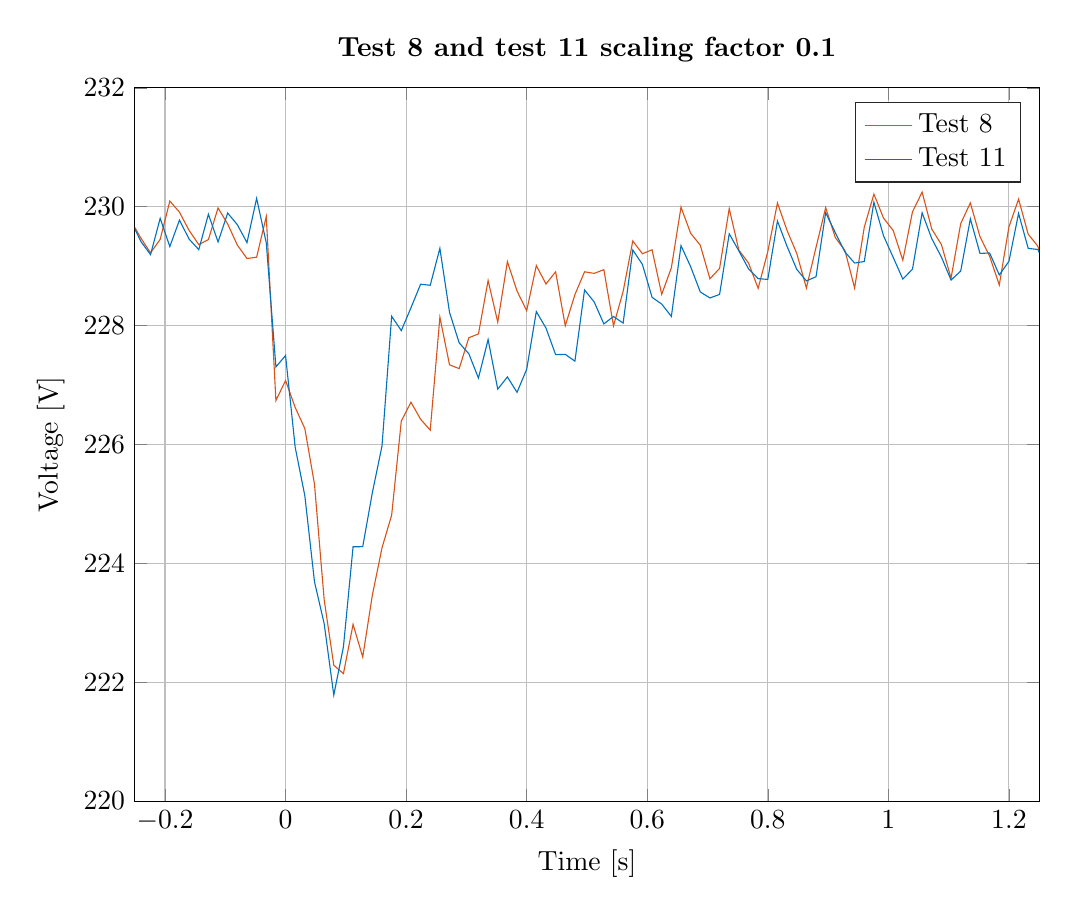
\begin{tikzpicture}

\begin{axis}[%
width=4.521in,
height=3.566in,
at={(0.758in,0.481in)},
scale only axis,
xmin=-0.25,
xmax=1.25,
xlabel={Time [s]},
xmajorgrids,
ymin=220,
ymax=232,
ylabel={Voltage [V]},
ymajorgrids,
axis background/.style={fill=white},
title style={font=\bfseries},
title={Test 8 and test 11 scaling factor 0.1},
legend style={legend cell align=left,align=left,draw=white!15!black}
]
\addplot [color=mycolor1,solid]
  table[row sep=crcr]{%
-0.256	229.755793228974\\
-0.240000000000002	229.471176350049\\
-0.224	229.223916811137\\
-0.208000000000002	229.450675310923\\
-0.192	230.095133045459\\
-0.176000000000002	229.908738814126\\
-0.16	229.601377967914\\
-0.144000000000002	229.362692002392\\
-0.128	229.447839011785\\
-0.112000000000002	229.979719521194\\
-0.0960000000000001	229.709497238476\\
-0.0800000000000018	229.35447493813\\
-0.0640000000000001	229.129044012428\\
-0.0480000000000018	229.151018521351\\
-0.032	229.835229873847\\
-0.0160000000000018	226.739456710433\\
0	227.076652901712\\
0.0159999999999982	226.621736785808\\
0.032	226.267135392901\\
0.0479999999999983	225.331035521847\\
0.0640000000000001	223.392136305783\\
0.0799999999999983	222.285649841967\\
0.0960000000000001	222.143981201873\\
0.111999999999998	222.972574249643\\
0.128	222.423906218219\\
0.143999999999998	223.465708954518\\
0.16	224.261390871722\\
0.175999999999998	224.811410086885\\
0.192	226.39378987966\\
0.207999999999998	226.711368418361\\
0.224	226.425221308128\\
0.239999999999998	226.240385743222\\
0.256	228.141464294356\\
0.271999999999998	227.340281442321\\
0.288	227.27651231268\\
0.303999999999998	227.795544408403\\
0.32	227.859997296007\\
0.335999999999999	228.759392523974\\
0.352	228.05813240013\\
0.367999999999999	229.076055509652\\
0.384	228.581911683237\\
0.399999999999999	228.250240475284\\
0.416	229.009836870942\\
0.431999999999999	228.700243731579\\
0.448	228.905071515245\\
0.463999999999999	227.996712525699\\
0.479999999999997	228.520954672748\\
0.495999999999999	228.905408835514\\
0.511999999999997	228.878605539116\\
0.527999999999999	228.941630373706\\
0.543999999999997	227.99589017644\\
0.559999999999999	228.574544995099\\
0.575999999999997	229.424321372088\\
0.591999999999999	229.209562164554\\
0.607999999999997	229.275315688313\\
0.623999999999999	228.526334060035\\
0.639999999999997	228.972585818592\\
0.655999999999999	229.992668916109\\
0.671999999999997	229.552908623312\\
0.687999999999999	229.352421759234\\
0.703999999999997	228.788025526098\\
0.719999999999999	228.961862509787\\
0.735999999999997	229.968964958511\\
0.751999999999999	229.26993568248\\
0.767999999999997	229.053001927011\\
0.783999999999999	228.627036490637\\
0.799999999999997	229.245265921995\\
0.815999999999999	230.063177722537\\
0.831999999999997	229.599759201865\\
0.847999999999999	229.215392681505\\
0.863999999999997	228.63317962675\\
0.879999999999999	229.316909651675\\
0.895999999999997	229.984674859096\\
0.911999999999999	229.481345336619\\
0.927999999999997	229.262980942599\\
0.943999999999999	228.632891151849\\
0.959999999999997	229.654450646327\\
0.975999999999999	230.211952810946\\
0.991999999999997	229.808758139791\\
1.008	229.600333375737\\
1.024	229.099669125591\\
1.04	229.914271820836\\
1.056	230.245498948148\\
1.072	229.624515241211\\
1.088	229.36378459628\\
1.104	228.799285275565\\
1.12	229.715668006143\\
1.136	230.064822815609\\
1.152	229.497208474902\\
1.168	229.166641486987\\
1.184	228.682880836958\\
1.2	229.660663396228\\
1.216	230.127240550322\\
1.232	229.537017288117\\
1.248	229.336196342122\\
1.264	228.738103493305\\
};
\addlegendentry{Test 8};

\addplot [color=mycolor2,solid]
  table[row sep=crcr]{%
-0.256	229.752903067837\\
-0.240000000000002	229.414654820608\\
-0.223999999999997	229.194842563361\\
-0.207999999999998	229.804821491914\\
-0.192	229.329593228241\\
-0.176000000000002	229.774552958348\\
-0.159999999999997	229.455402773706\\
-0.143999999999998	229.277710490583\\
-0.128	229.87319726138\\
-0.112000000000002	229.408932026939\\
-0.0959999999999965	229.893952010505\\
-0.0799999999999983	229.697961288075\\
-0.0640000000000001	229.396135463738\\
-0.0480000000000018	230.141122260726\\
-0.0319999999999965	229.392447703964\\
-0.0159999999999982	227.304694968184\\
0	227.496904206485\\
0.0159999999999982	225.950911703511\\
0.0320000000000036	225.135482375551\\
0.0480000000000018	223.689198213333\\
0.0640000000000001	222.987694788874\\
0.0799999999999983	221.784368702369\\
0.0960000000000036	222.594704655994\\
0.112000000000002	224.279313523938\\
0.128	224.280340384068\\
0.143999999999998	225.189701270275\\
0.160000000000004	225.975425308018\\
0.176000000000002	228.156750690921\\
0.192	227.915763137658\\
0.207999999999998	228.299267428293\\
0.224000000000004	228.69622543526\\
0.240000000000002	228.678695271503\\
0.256	229.299744662446\\
0.271999999999998	228.223603062439\\
0.288000000000004	227.710236453603\\
0.304000000000002	227.527008423222\\
0.32	227.116348554616\\
0.335999999999999	227.765307655362\\
0.352000000000004	226.930694997868\\
0.368000000000002	227.136287192649\\
0.384	226.877550309032\\
0.399999999999999	227.264855625753\\
0.416000000000004	228.235816844724\\
0.432000000000002	227.958998345186\\
0.448	227.511284418686\\
0.463999999999999	227.516146533013\\
0.480000000000004	227.401585252906\\
0.496000000000002	228.600053620825\\
0.512	228.397904508039\\
0.527999999999999	228.028529257136\\
0.544000000000004	228.153021339521\\
0.560000000000002	228.042354186992\\
0.576000000000001	229.271423628023\\
0.591999999999999	229.028264228141\\
0.608000000000004	228.476006651239\\
0.624000000000002	228.362027704631\\
0.640000000000001	228.154180640517\\
0.655999999999999	229.345715847805\\
0.672000000000004	228.991213466229\\
0.688000000000002	228.566079452006\\
0.704000000000001	228.465331589787\\
0.719999999999999	228.524660119802\\
0.736000000000004	229.543681516169\\
0.752000000000002	229.257154621666\\
0.768000000000001	228.95570884183\\
0.783999999999999	228.789910041775\\
0.800000000000004	228.777156490574\\
0.816000000000003	229.758468915827\\
0.832000000000001	229.332084525903\\
0.847999999999999	228.947162855242\\
0.864000000000004	228.75191271622\\
0.880000000000003	228.822342087829\\
0.896000000000001	229.900587074409\\
0.911999999999999	229.562927915232\\
0.928000000000004	229.237679002378\\
0.944000000000003	229.052886273561\\
0.960000000000001	229.078130556405\\
0.975999999999999	230.076448958427\\
0.992000000000004	229.510207513044\\
1.008	229.148589474516\\
1.024	228.782245153754\\
1.04	228.949849043008\\
1.056	229.897620865973\\
1.072	229.463414826347\\
1.088	229.152985180255\\
1.104	228.766975826071\\
1.12	228.917322866854\\
1.136	229.796815935214\\
1.152	229.214587903364\\
1.168	229.22168403585\\
1.184	228.852884960631\\
1.2	229.080783966382\\
1.216	229.887814960419\\
1.232	229.298733426657\\
1.248	229.281259761375\\
1.264	228.922048755422\\
};
\addlegendentry{Test 11};
\end{axis}
\end{tikzpicture}%
\caption{Step from 20 to 30 kW load. }
\label{fig:test8+11volt20-30kwstep}
\end{figure}


\begin{figure}[H]
\centering
% This file was created by matlab2tikz.
%
%The latest updates can be retrieved from
%  http://www.mathworks.com/matlabcentral/fileexchange/22022-matlab2tikz-matlab2tikz
%where you can also make suggestions and rate matlab2tikz.
%
\definecolor{mycolor1}{rgb}{0.00000,0.44700,0.74100}%
\definecolor{mycolor2}{rgb}{0.85000,0.32500,0.09800}%
%
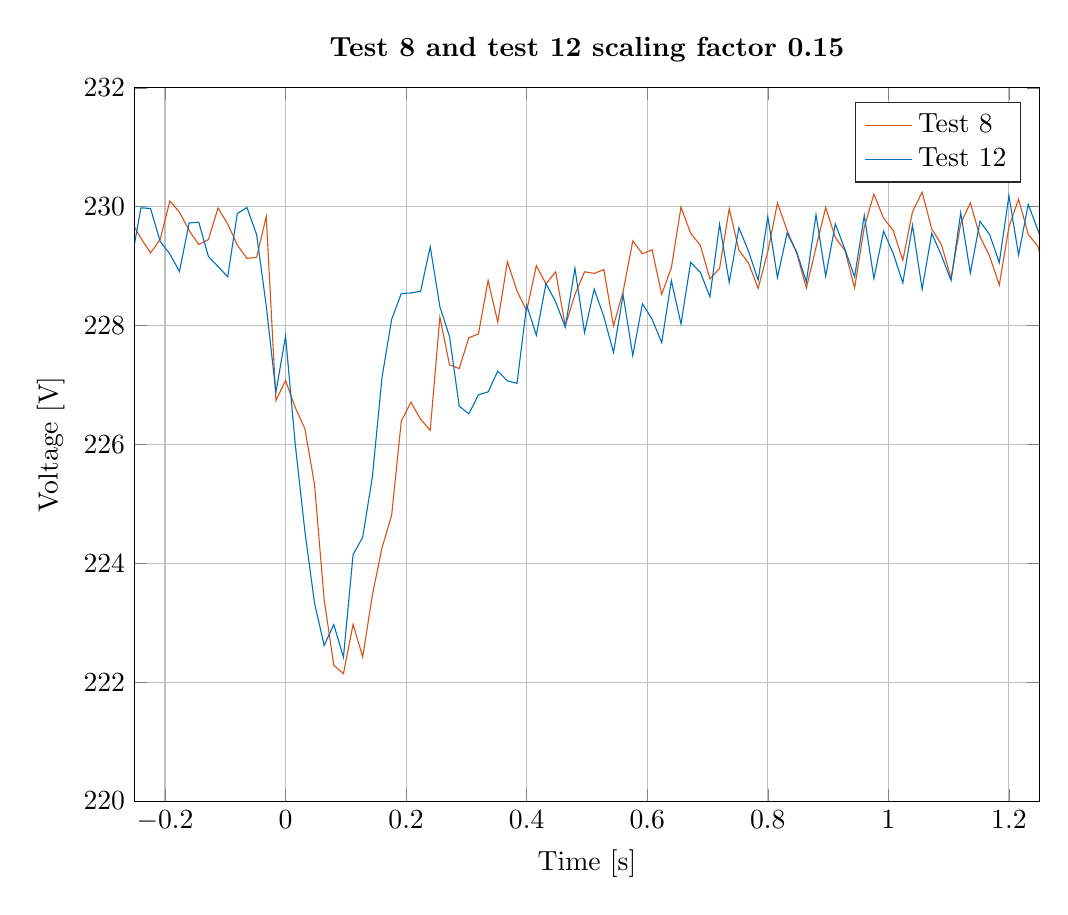
\begin{tikzpicture}

\begin{axis}[%
width=4.521in,
height=3.566in,
at={(0.758in,0.481in)},
scale only axis,
xmin=-0.25,
xmax=1.25,
xlabel={Time [s]},
xmajorgrids,
ymin=220,
ymax=232,
ylabel={Voltage [V]},
ymajorgrids,
axis background/.style={fill=white},
title style={font=\bfseries},
title={Test 8 and test 12 scaling factor 0.15},
legend style={legend cell align=left,align=left,draw=white!15!black}
]
\addplot [color=mycolor1,solid]
  table[row sep=crcr]{%
-0.256	229.755793228974\\
-0.240000000000002	229.471176350049\\
-0.224	229.223916811137\\
-0.208000000000002	229.450675310923\\
-0.192	230.095133045459\\
-0.176000000000002	229.908738814126\\
-0.16	229.601377967914\\
-0.144000000000002	229.362692002392\\
-0.128	229.447839011785\\
-0.112000000000002	229.979719521194\\
-0.0960000000000001	229.709497238476\\
-0.0800000000000018	229.35447493813\\
-0.0640000000000001	229.129044012428\\
-0.0480000000000018	229.151018521351\\
-0.032	229.835229873847\\
-0.0160000000000018	226.739456710433\\
0	227.076652901712\\
0.0159999999999982	226.621736785808\\
0.032	226.267135392901\\
0.0479999999999983	225.331035521847\\
0.0640000000000001	223.392136305783\\
0.0799999999999983	222.285649841967\\
0.0960000000000001	222.143981201873\\
0.111999999999998	222.972574249643\\
0.128	222.423906218219\\
0.143999999999998	223.465708954518\\
0.16	224.261390871722\\
0.175999999999998	224.811410086885\\
0.192	226.39378987966\\
0.207999999999998	226.711368418361\\
0.224	226.425221308128\\
0.239999999999998	226.240385743222\\
0.256	228.141464294356\\
0.271999999999998	227.340281442321\\
0.288	227.27651231268\\
0.303999999999998	227.795544408403\\
0.32	227.859997296007\\
0.335999999999999	228.759392523974\\
0.352	228.05813240013\\
0.367999999999999	229.076055509652\\
0.384	228.581911683237\\
0.399999999999999	228.250240475284\\
0.416	229.009836870942\\
0.431999999999999	228.700243731579\\
0.448	228.905071515245\\
0.463999999999999	227.996712525699\\
0.479999999999997	228.520954672748\\
0.495999999999999	228.905408835514\\
0.511999999999997	228.878605539116\\
0.527999999999999	228.941630373706\\
0.543999999999997	227.99589017644\\
0.559999999999999	228.574544995099\\
0.575999999999997	229.424321372088\\
0.591999999999999	229.209562164554\\
0.607999999999997	229.275315688313\\
0.623999999999999	228.526334060035\\
0.639999999999997	228.972585818592\\
0.655999999999999	229.992668916109\\
0.671999999999997	229.552908623312\\
0.687999999999999	229.352421759234\\
0.703999999999997	228.788025526098\\
0.719999999999999	228.961862509787\\
0.735999999999997	229.968964958511\\
0.751999999999999	229.26993568248\\
0.767999999999997	229.053001927011\\
0.783999999999999	228.627036490637\\
0.799999999999997	229.245265921995\\
0.815999999999999	230.063177722537\\
0.831999999999997	229.599759201865\\
0.847999999999999	229.215392681505\\
0.863999999999997	228.63317962675\\
0.879999999999999	229.316909651675\\
0.895999999999997	229.984674859096\\
0.911999999999999	229.481345336619\\
0.927999999999997	229.262980942599\\
0.943999999999999	228.632891151849\\
0.959999999999997	229.654450646327\\
0.975999999999999	230.211952810946\\
0.991999999999997	229.808758139791\\
1.008	229.600333375737\\
1.024	229.099669125591\\
1.04	229.914271820836\\
1.056	230.245498948148\\
1.072	229.624515241211\\
1.088	229.36378459628\\
1.104	228.799285275565\\
1.12	229.715668006143\\
1.136	230.064822815609\\
1.152	229.497208474902\\
1.168	229.166641486987\\
1.184	228.682880836958\\
1.2	229.660663396228\\
1.216	230.127240550322\\
1.232	229.537017288117\\
1.248	229.336196342122\\
1.264	228.738103493305\\
};
\addlegendentry{Test 8};

\addplot [color=mycolor2,solid]
  table[row sep=crcr]{%
-0.256	229.067772664087\\
-0.240000000000002	229.981303177857\\
-0.223999999999997	229.970640468476\\
-0.207999999999998	229.416721684474\\
-0.192	229.205158395487\\
-0.176000000000002	228.911161022096\\
-0.159999999999997	229.727186538087\\
-0.143999999999998	229.739475458563\\
-0.128	229.163572272113\\
-0.112000000000002	228.993183302376\\
-0.0959999999999965	228.820438107189\\
-0.0799999999999983	229.887046968764\\
-0.0640000000000001	229.986817580974\\
-0.0480000000000018	229.530757532312\\
-0.0319999999999965	228.328766370483\\
-0.0159999999999982	226.878049952568\\
0	227.826189382336\\
0.0159999999999982	226.008231975321\\
0.0320000000000036	224.543917613826\\
0.0480000000000018	223.333632448495\\
0.0640000000000001	222.619039680968\\
0.0799999999999983	222.970061198068\\
0.0959999999999965	222.420758046394\\
0.112000000000002	224.14520643257\\
0.128	224.441960452128\\
0.143999999999998	225.453455140723\\
0.159999999999997	227.12764012726\\
0.176000000000002	228.106651389528\\
0.192	228.540891897199\\
0.207999999999998	228.548559529131\\
0.223999999999997	228.579057663034\\
0.240000000000002	229.324754313279\\
0.256	228.317428976695\\
0.271999999999998	227.817453633184\\
0.287999999999997	226.645790142356\\
0.304000000000002	226.515471760768\\
0.32	226.836052015981\\
0.335999999999999	226.884149695196\\
0.351999999999997	227.234185116208\\
0.368000000000002	227.071406321448\\
0.384	227.028459712305\\
0.399999999999999	228.344939397915\\
0.415999999999997	227.838461383182\\
0.432000000000002	228.706950031725\\
0.448	228.400784647715\\
0.463999999999999	227.973932430586\\
0.479999999999997	228.964824915987\\
0.496000000000002	227.882065427547\\
0.512	228.613726047436\\
0.527999999999999	228.150234652435\\
0.543999999999997	227.548481271938\\
0.560000000000002	228.516227513726\\
0.576000000000001	227.496073230538\\
0.591999999999999	228.367732235235\\
0.607999999999997	228.108376484968\\
0.624000000000002	227.713877708019\\
0.640000000000001	228.756431069643\\
0.655999999999999	228.029720945102\\
0.671999999999997	229.064590023181\\
0.688000000000002	228.896266378989\\
0.704000000000001	228.485771798654\\
0.719999999999999	229.705782171109\\
0.735999999999997	228.726736283592\\
0.752000000000002	229.645572294705\\
0.768000000000001	229.253457271228\\
0.783999999999999	228.764436412669\\
0.799999999999997	229.832582597374\\
0.816000000000003	228.808749261809\\
0.832000000000001	229.556769885615\\
0.847999999999999	229.236761939462\\
0.863999999999997	228.737749854885\\
0.880000000000003	229.866506893853\\
0.896000000000001	228.831264169166\\
0.911999999999999	229.710376429402\\
0.927999999999997	229.280681644449\\
0.944000000000003	228.819824446882\\
0.960000000000001	229.852034886811\\
0.975999999999999	228.793265941422\\
0.991999999999997	229.587145123287\\
1.008	229.216368215215\\
1.024	228.717828463923\\
1.04	229.687284069901\\
1.056	228.613774838562\\
1.072	229.551307749498\\
1.088	229.181491116801\\
1.104	228.757943987876\\
1.12	229.899158242521\\
1.136	228.885833971242\\
1.152	229.753776282206\\
1.168	229.532290272094\\
1.184	229.05943466392\\
1.2	230.187148041988\\
1.216	229.188848757901\\
1.232	230.040510495071\\
1.248	229.610888989085\\
1.264	229.136195221385\\
};
\addlegendentry{Test 12};
\end{axis}
\end{tikzpicture}%
\caption{Step from 20 to 30 kW load. }
\label{fig:test8+12volt20-30kwstep}
\end{figure}

\begin{figure}[H]
\centering
% This file was created by matlab2tikz.
%
%The latest updates can be retrieved from
%  http://www.mathworks.com/matlabcentral/fileexchange/22022-matlab2tikz-matlab2tikz
%where you can also make suggestions and rate matlab2tikz.
%
\definecolor{mycolor1}{rgb}{0.00000,0.44700,0.74100}%
\definecolor{mycolor2}{rgb}{0.85000,0.32500,0.09800}%
%
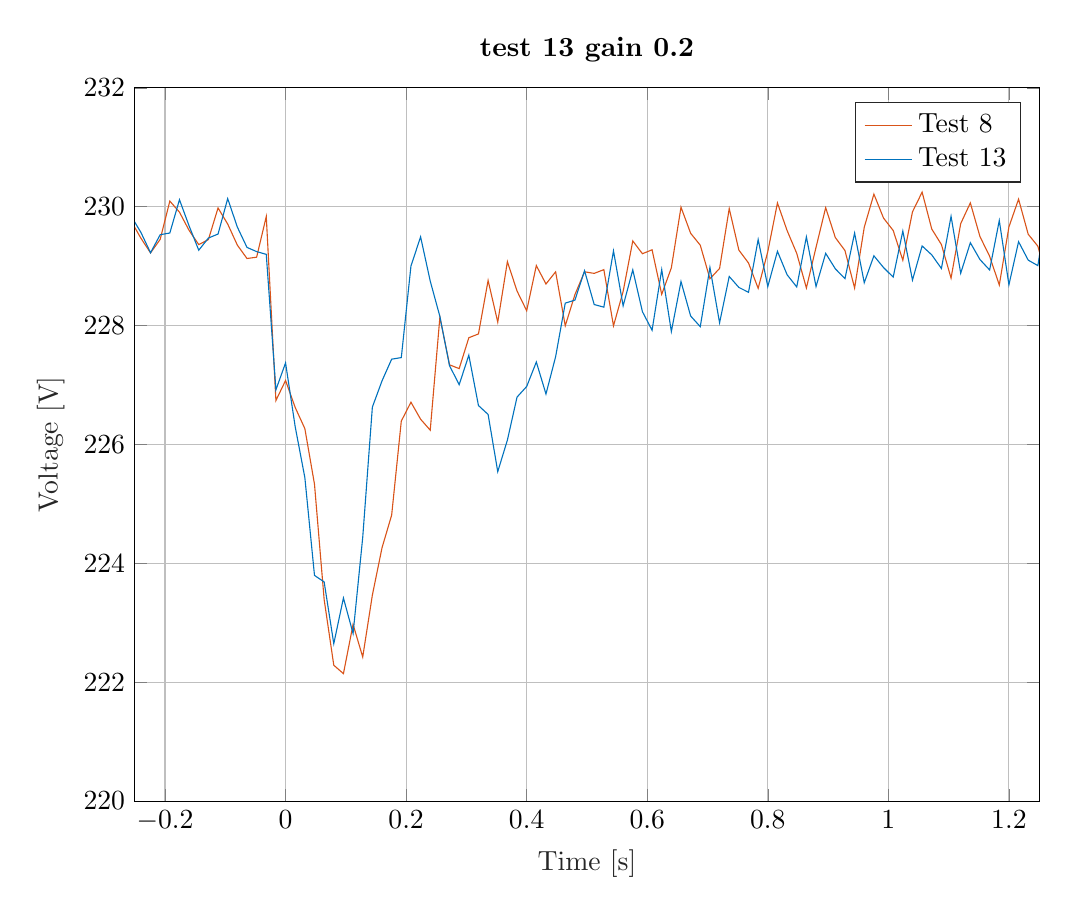
\begin{tikzpicture}

\begin{axis}[%
width=4.521in,
height=3.566in,
at={(0.758in,0.481in)},
scale only axis,
xmin=-0.25,
xmax=1.25,
xlabel style={font=\color{white!15!black}},
xlabel={Time [s]},
xmajorgrids,
ymin=220,
ymax=232,
ylabel style={font=\color{white!15!black}},
ylabel={Voltage [V]},
ymajorgrids,
axis background/.style={fill=white},
title style={font=\bfseries},
title={test 13  gain 0.2},
legend style={legend cell align=left, align=left, draw=white!15!black}
]
\addplot [color=mycolor1]
  table[row sep=crcr]{%
-0.256	229.755793228974\\
-0.240000000000009	229.471176350049\\
-0.22399999999999	229.223916811137\\
-0.207999999999998	229.450675310923\\
-0.192000000000007	230.095133045459\\
-0.176000000000016	229.908738814126\\
-0.159999999999997	229.601377967914\\
-0.144000000000005	229.362692002392\\
-0.128000000000014	229.447839011785\\
-0.111999999999995	229.979719521194\\
-0.0960000000000036	229.709497238476\\
-0.0800000000000125	229.35447493813\\
-0.063999999999993	229.129044012428\\
-0.0480000000000018	229.151018521351\\
-0.0320000000000107	229.835229873847\\
-0.0159999999999911	226.739456710433\\
0	227.076652901712\\
0.0159999999999911	226.621736785808\\
0.0320000000000107	226.267135392901\\
0.0480000000000018	225.331035521847\\
0.063999999999993	223.392136305783\\
0.0800000000000125	222.285649841967\\
0.0960000000000036	222.143981201873\\
0.111999999999995	222.972574249643\\
0.128000000000014	222.423906218219\\
0.144000000000005	223.465708954518\\
0.159999999999997	224.261390871722\\
0.175999999999988	224.811410086885\\
0.192000000000007	226.39378987966\\
0.207999999999998	226.711368418361\\
0.22399999999999	226.425221308128\\
0.240000000000009	226.240385743222\\
0.256	228.141464294356\\
0.271999999999991	227.340281442321\\
0.288000000000011	227.27651231268\\
0.304000000000002	227.795544408403\\
0.319999999999993	227.859997296007\\
0.336000000000013	228.759392523974\\
0.352000000000004	228.05813240013\\
0.367999999999995	229.076055509652\\
0.384000000000015	228.581911683237\\
0.400000000000006	228.250240475284\\
0.415999999999997	229.009836870942\\
0.431999999999988	228.700243731579\\
0.448000000000008	228.905071515245\\
0.463999999999999	227.996712525699\\
0.47999999999999	228.520954672748\\
0.496000000000009	228.905408835514\\
0.512	228.878605539116\\
0.527999999999992	228.941630373706\\
0.544000000000011	227.99589017644\\
0.560000000000002	228.574544995099\\
0.575999999999993	229.424321372088\\
0.592000000000013	229.209562164554\\
0.608000000000004	229.275315688313\\
0.623999999999995	228.526334060035\\
0.639999999999986	228.972585818592\\
0.656000000000006	229.992668916109\\
0.671999999999997	229.552908623312\\
0.687999999999988	229.352421759234\\
0.704000000000008	228.788025526098\\
0.719999999999999	228.961862509787\\
0.73599999999999	229.968964958511\\
0.75200000000001	229.26993568248\\
0.768000000000001	229.053001927011\\
0.783999999999992	228.627036490637\\
0.800000000000011	229.245265921995\\
0.816000000000003	230.063177722537\\
0.831999999999994	229.599759201865\\
0.848000000000013	229.215392681505\\
0.864000000000004	228.63317962675\\
0.879999999999995	229.316909651675\\
0.895999999999987	229.984674859096\\
0.912000000000006	229.481345336619\\
0.927999999999997	229.262980942599\\
0.943999999999988	228.632891151849\\
0.960000000000008	229.654450646327\\
0.975999999999999	230.211952810946\\
0.99199999999999	229.808758139791\\
1.00800000000001	229.600333375737\\
1.024	229.099669125591\\
1.03999999999999	229.914271820836\\
1.05600000000001	230.245498948148\\
1.072	229.624515241211\\
1.08799999999999	229.36378459628\\
1.10400000000001	228.799285275565\\
1.12	229.715668006143\\
1.136	230.064822815609\\
1.15199999999999	229.497208474902\\
1.16800000000001	229.166641486987\\
1.184	228.682880836958\\
1.19999999999999	229.660663396228\\
1.21600000000001	230.127240550322\\
1.232	229.537017288117\\
1.24799999999999	229.336196342122\\
1.26400000000001	228.738103493305\\
};
\addlegendentry{Test 8}

\addplot [color=mycolor2, solid]
  table[row sep=crcr]{%
-0.256	229.839517999578\\
-0.240000000000009	229.569354256343\\
-0.224000000000018	229.225389733922\\
-0.207999999999998	229.52947252264\\
-0.192000000000007	229.558011945168\\
-0.176000000000016	230.11815738\\
-0.159999999999997	229.676675428709\\
-0.144000000000005	229.268320376002\\
-0.128000000000014	229.473297216628\\
-0.111999999999995	229.540821104572\\
-0.0960000000000036	230.136359913018\\
-0.0800000000000125	229.658160008794\\
-0.0640000000000214	229.315808934168\\
-0.0480000000000018	229.245136418843\\
-0.0320000000000107	229.198644109513\\
-0.0160000000000196	226.920032228587\\
-0	227.372223276296\\
0.0159999999999911	226.297794285725\\
0.0320000000000107	225.442403693893\\
0.0480000000000018	223.796978298177\\
0.063999999999993	223.687598964528\\
0.0799999999999841	222.648176349269\\
0.0960000000000036	223.41691931648\\
0.111999999999995	222.819521955293\\
0.127999999999986	224.435729283819\\
0.144000000000005	226.628669541771\\
0.159999999999997	227.06958309546\\
0.175999999999988	227.435440280114\\
0.192000000000007	227.461742037251\\
0.207999999999998	229.000961599663\\
0.22399999999999	229.493750944467\\
0.240000000000009	228.748887985251\\
0.256	228.154737192644\\
0.271999999999991	227.326358886315\\
0.288000000000011	227.005630184309\\
0.304000000000002	227.502009650897\\
0.319999999999993	226.655153119979\\
0.335999999999984	226.505214652445\\
0.352000000000004	225.542909393759\\
0.367999999999995	226.07363199443\\
0.383999999999986	226.797134730408\\
0.400000000000006	226.97563642231\\
0.415999999999997	227.387424026518\\
0.431999999999988	226.849088771048\\
0.448000000000008	227.47623613869\\
0.463999999999999	228.378177230764\\
0.47999999999999	228.428784341785\\
0.496000000000009	228.923439712505\\
0.512	228.354447795014\\
0.527999999999992	228.310498993267\\
0.544000000000011	229.256645261146\\
0.560000000000002	228.332535924791\\
0.575999999999993	228.9378554606\\
0.591999999999985	228.234852171997\\
0.608000000000004	227.921264421621\\
0.623999999999995	228.941655888312\\
0.639999999999986	227.900513335464\\
0.656000000000006	228.741471874977\\
0.671999999999997	228.161157552633\\
0.687999999999988	227.981917442093\\
0.704000000000008	228.978488215934\\
0.719999999999999	228.047269157798\\
0.73599999999999	228.826656327532\\
0.75200000000001	228.642289416232\\
0.768000000000001	228.560831903894\\
0.783999999999992	229.447946253844\\
0.800000000000011	228.657789047373\\
0.816000000000003	229.249691515758\\
0.831999999999994	228.855821698572\\
0.847999999999985	228.650255278497\\
0.864000000000004	229.492498676097\\
0.879999999999995	228.656736846718\\
0.895999999999987	229.215717137212\\
0.912000000000006	228.955714292449\\
0.927999999999997	228.790124385448\\
0.943999999999988	229.556297749959\\
0.960000000000008	228.721417763147\\
0.975999999999999	229.174751475618\\
0.99199999999999	228.976284983403\\
1.00800000000001	228.815851064887\\
1.024	229.591196803545\\
1.03999999999999	228.765713019338\\
1.05600000000001	229.340105528993\\
1.072	229.18977623437\\
1.08799999999999	228.961022009178\\
1.10399999999999	229.839302900309\\
1.12	228.88134774087\\
1.136	229.39462624968\\
1.15199999999999	229.110681031734\\
1.16800000000001	228.93619117106\\
1.184	229.768094888508\\
1.19999999999999	228.686293487702\\
1.21600000000001	229.411174911615\\
1.232	229.101456793359\\
1.24799999999999	229.009395362797\\
1.26400000000001	230.023206632665\\
};
\addlegendentry{Test 13}
\end{axis}
\end{tikzpicture}%
\caption{Step from 20 to 30 kW load. }
\label{fig:test8+13volt20-30kwstep}
\end{figure}

\begin{figure}[H]
\centering
% This file was created by matlab2tikz.
%
%The latest updates can be retrieved from
%  http://www.mathworks.com/matlabcentral/fileexchange/22022-matlab2tikz-matlab2tikz
%where you can also make suggestions and rate matlab2tikz.
%
\definecolor{mycolor1}{rgb}{0.00000,0.44700,0.74100}%
\definecolor{mycolor2}{rgb}{0.85000,0.32500,0.09800}%
%
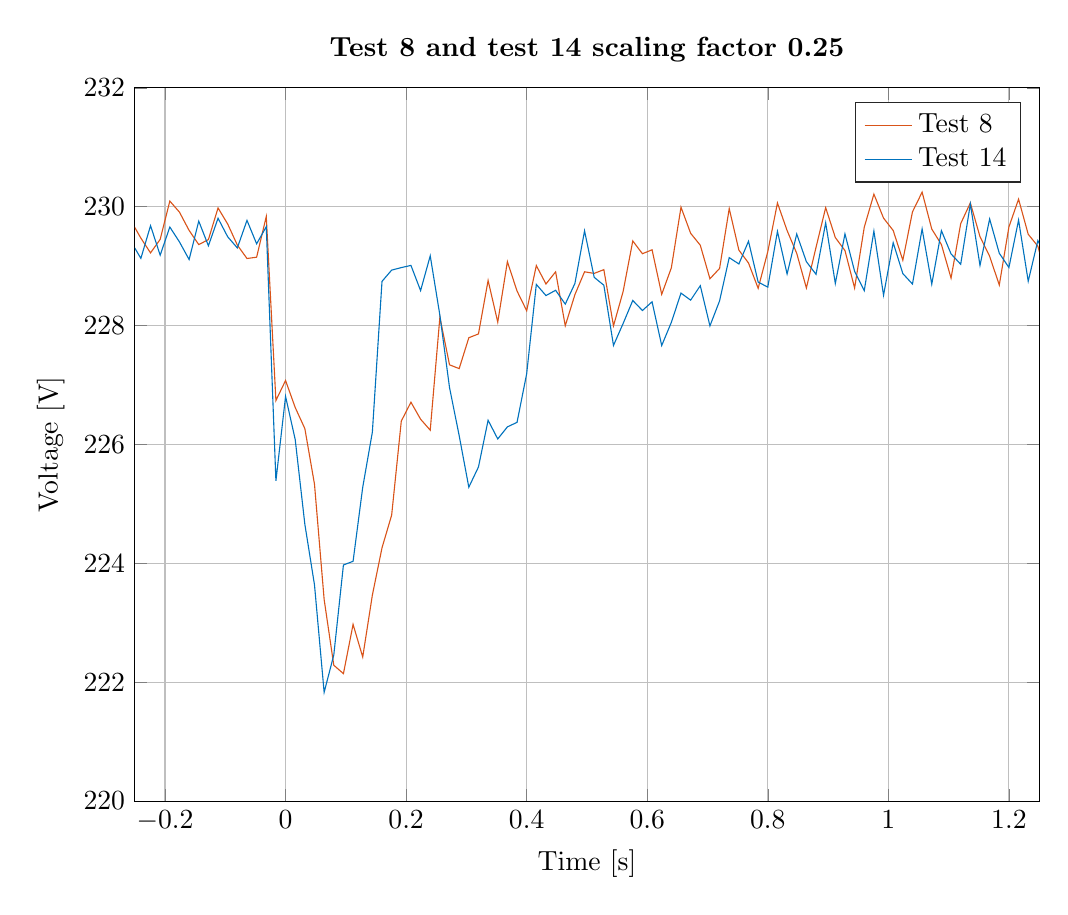
\begin{tikzpicture}

\begin{axis}[%
width=4.521in,
height=3.566in,
at={(0.758in,0.481in)},
scale only axis,
xmin=-0.25,
xmax=1.25,
xlabel={Time [s]},
xmajorgrids,
ymin=220,
ymax=232,
ylabel={Voltage [V]},
ymajorgrids,
axis background/.style={fill=white},
title style={font=\bfseries},
title={Test 8 and test 14 scaling factor 0.25},
legend style={legend cell align=left,align=left,draw=white!15!black}
]
\addplot [color=mycolor1,solid]
  table[row sep=crcr]{%
-0.256	229.755793228974\\
-0.240000000000002	229.471176350049\\
-0.224	229.223916811137\\
-0.208000000000002	229.450675310923\\
-0.192	230.095133045459\\
-0.176000000000002	229.908738814126\\
-0.16	229.601377967914\\
-0.144000000000002	229.362692002392\\
-0.128	229.447839011785\\
-0.112000000000002	229.979719521194\\
-0.0960000000000001	229.709497238476\\
-0.0800000000000018	229.35447493813\\
-0.0640000000000001	229.129044012428\\
-0.0480000000000018	229.151018521351\\
-0.032	229.835229873847\\
-0.0160000000000018	226.739456710433\\
0	227.076652901712\\
0.0159999999999982	226.621736785808\\
0.032	226.267135392901\\
0.0479999999999983	225.331035521847\\
0.0640000000000001	223.392136305783\\
0.0799999999999983	222.285649841967\\
0.0960000000000001	222.143981201873\\
0.111999999999998	222.972574249643\\
0.128	222.423906218219\\
0.143999999999998	223.465708954518\\
0.16	224.261390871722\\
0.175999999999998	224.811410086885\\
0.192	226.39378987966\\
0.207999999999998	226.711368418361\\
0.224	226.425221308128\\
0.239999999999998	226.240385743222\\
0.256	228.141464294356\\
0.271999999999998	227.340281442321\\
0.288	227.27651231268\\
0.303999999999998	227.795544408403\\
0.32	227.859997296007\\
0.335999999999999	228.759392523974\\
0.352	228.05813240013\\
0.367999999999999	229.076055509652\\
0.384	228.581911683237\\
0.399999999999999	228.250240475284\\
0.416	229.009836870942\\
0.431999999999999	228.700243731579\\
0.448	228.905071515245\\
0.463999999999999	227.996712525699\\
0.479999999999997	228.520954672748\\
0.495999999999999	228.905408835514\\
0.511999999999997	228.878605539116\\
0.527999999999999	228.941630373706\\
0.543999999999997	227.99589017644\\
0.559999999999999	228.574544995099\\
0.575999999999997	229.424321372088\\
0.591999999999999	229.209562164554\\
0.607999999999997	229.275315688313\\
0.623999999999999	228.526334060035\\
0.639999999999997	228.972585818592\\
0.655999999999999	229.992668916109\\
0.671999999999997	229.552908623312\\
0.687999999999999	229.352421759234\\
0.703999999999997	228.788025526098\\
0.719999999999999	228.961862509787\\
0.735999999999997	229.968964958511\\
0.751999999999999	229.26993568248\\
0.767999999999997	229.053001927011\\
0.783999999999999	228.627036490637\\
0.799999999999997	229.245265921995\\
0.815999999999999	230.063177722537\\
0.831999999999997	229.599759201865\\
0.847999999999999	229.215392681505\\
0.863999999999997	228.63317962675\\
0.879999999999999	229.316909651675\\
0.895999999999997	229.984674859096\\
0.911999999999999	229.481345336619\\
0.927999999999997	229.262980942599\\
0.943999999999999	228.632891151849\\
0.959999999999997	229.654450646327\\
0.975999999999999	230.211952810946\\
0.991999999999997	229.808758139791\\
1.008	229.600333375737\\
1.024	229.099669125591\\
1.04	229.914271820836\\
1.056	230.245498948148\\
1.072	229.624515241211\\
1.088	229.36378459628\\
1.104	228.799285275565\\
1.12	229.715668006143\\
1.136	230.064822815609\\
1.152	229.497208474902\\
1.168	229.166641486987\\
1.184	228.682880836958\\
1.2	229.660663396228\\
1.216	230.127240550322\\
1.232	229.537017288117\\
1.248	229.336196342122\\
1.264	228.738103493305\\
};
\addlegendentry{Test 8};

\addplot [color=mycolor2,solid]
  table[row sep=crcr]{%
-0.256	229.404378361467\\
-0.240000000000002	229.131400560786\\
-0.224000000000004	229.681642000366\\
-0.208000000000006	229.185056904661\\
-0.192	229.658365960582\\
-0.176000000000002	229.407636041154\\
-0.160000000000004	229.111976406294\\
-0.144000000000005	229.757178303865\\
-0.128	229.34312867851\\
-0.112000000000002	229.806494779953\\
-0.0960000000000036	229.494321760796\\
-0.0800000000000054	229.306968618558\\
-0.0640000000000001	229.770924461604\\
-0.0480000000000018	229.376273082785\\
-0.0320000000000036	229.663482838238\\
-0.0160000000000053	225.387762884078\\
0	226.80884986918\\
0.0159999999999982	226.083359785976\\
0.0319999999999965	224.657586352954\\
0.0479999999999947	223.637006438344\\
0.0640000000000001	221.829645945769\\
0.0799999999999983	222.45739996485\\
0.0959999999999965	223.972488444313\\
0.111999999999995	224.034232770866\\
0.128	225.279346895725\\
0.143999999999998	226.208330678125\\
0.159999999999997	228.744249836199\\
0.175999999999995	228.933768553703\\
0.192	228.976014596025\\
0.207999999999998	229.012962992864\\
0.223999999999997	228.58867958222\\
0.239999999999995	229.174092896441\\
0.256	228.17442074178\\
0.271999999999998	226.95751943009\\
0.287999999999997	226.148938346549\\
0.303999999999995	225.281020757945\\
0.32	225.620853131988\\
0.335999999999999	226.407437346891\\
0.351999999999997	226.093211483943\\
0.367999999999995	226.295984623321\\
0.384	226.37209020371\\
0.399999999999999	227.190878903155\\
0.415999999999997	228.693127471727\\
0.431999999999995	228.50543469757\\
0.447999999999993	228.594506011878\\
0.463999999999999	228.361361762937\\
0.479999999999997	228.709130121168\\
0.495999999999995	229.594329474504\\
0.511999999999993	228.812298873925\\
0.527999999999999	228.679739622833\\
0.543999999999997	227.666138627502\\
0.559999999999995	228.036012777906\\
0.575999999999993	228.422941219803\\
0.591999999999999	228.254100106078\\
0.607999999999997	228.400483820158\\
0.623999999999995	227.664550661041\\
0.639999999999993	228.055292342949\\
0.655999999999999	228.546808289311\\
0.671999999999997	228.428245553334\\
0.687999999999995	228.671661181272\\
0.703999999999994	227.99496270698\\
0.719999999999999	228.415769884734\\
0.735999999999997	229.144100528119\\
0.751999999999995	229.036929668334\\
0.767999999999994	229.419226922602\\
0.783999999999999	228.732026752328\\
0.799999999999997	228.647532740716\\
0.815999999999995	229.585282491676\\
0.831999999999994	228.868497844625\\
0.847999999999999	229.540063201803\\
0.863999999999997	229.075978134891\\
0.879999999999995	228.862712618532\\
0.895999999999994	229.72968792797\\
0.911999999999999	228.709446221416\\
0.927999999999997	229.542687837813\\
0.943999999999996	228.914130134147\\
0.959999999999994	228.587360208653\\
0.975999999999999	229.59045209963\\
0.991999999999997	228.511286550626\\
1.008	229.394720848644\\
1.02399999999999	228.875277853205\\
1.04	228.699441234647\\
1.056	229.626263752553\\
1.072	228.697777676665\\
1.08799999999999	229.597520296975\\
1.104	229.206284862734\\
1.12	229.031992474639\\
1.136	230.04674453355\\
1.15199999999999	229.01250345539\\
1.168	229.794239518555\\
1.184	229.218009307533\\
1.2	228.977556857717\\
1.21599999999999	229.77534771113\\
1.232	228.746409066881\\
1.248	229.430446639048\\
1.264	229.114193613807\\
};
\addlegendentry{Test 14};
\end{axis}
\end{tikzpicture}%
\caption{Step from 20 to 30 kW load. }
\label{fig:test8+14volt20-30kwstep}
\end{figure}


On \figref{fig:test8+11volt20-30kwstep} it is shown that the genset rises faster from a drop in voltage due to a load change with controller than without. %Both systems seems to reach steady state at the same time though, and a reason for this could be the second order model that the controller is designed for. 
Furthermore the step on the genset with controller shown on \figref{fig:test8+14volt20-30kwstep} reveals the characteristic similar to the second order model estimated in \secref{modelling_diesel_generator} and shown on \figref{fig:modelfreq_volt}, which occurs when the scaling factor is increased.


On figure \ref{fig:test8+11freq10to20kwstep}, \ref{fig:test8+12freq10to20kwstep}, \ref{fig:test8+13freq10to20kwstep} and \ref{fig:test8+14freq10to20kwstep} it is illustrated how the frequency changes when a step in the load from 10 to 20 kW is applied with different scaling factors. %It is shown that the genset with controller recovers faster to a change in load and thereby reach steady state before the genset without controller. 
For all four measurements it is shown that the genset with controller is less affected in frequency by the applied load steps, but at the cost of some overshoot. 
%The measuring data shown in figure \ref{fig:test8+11freq10to20kwstep}

   
\begin{figure}[H]
\centering
% This file was created by matlab2tikz.
%
%The latest updates can be retrieved from
%  http://www.mathworks.com/matlabcentral/fileexchange/22022-matlab2tikz-matlab2tikz
%where you can also make suggestions and rate matlab2tikz.
%
\definecolor{mycolor1}{rgb}{0.00000,0.44700,0.74100}%
\definecolor{mycolor2}{rgb}{0.85000,0.32500,0.09800}%
%
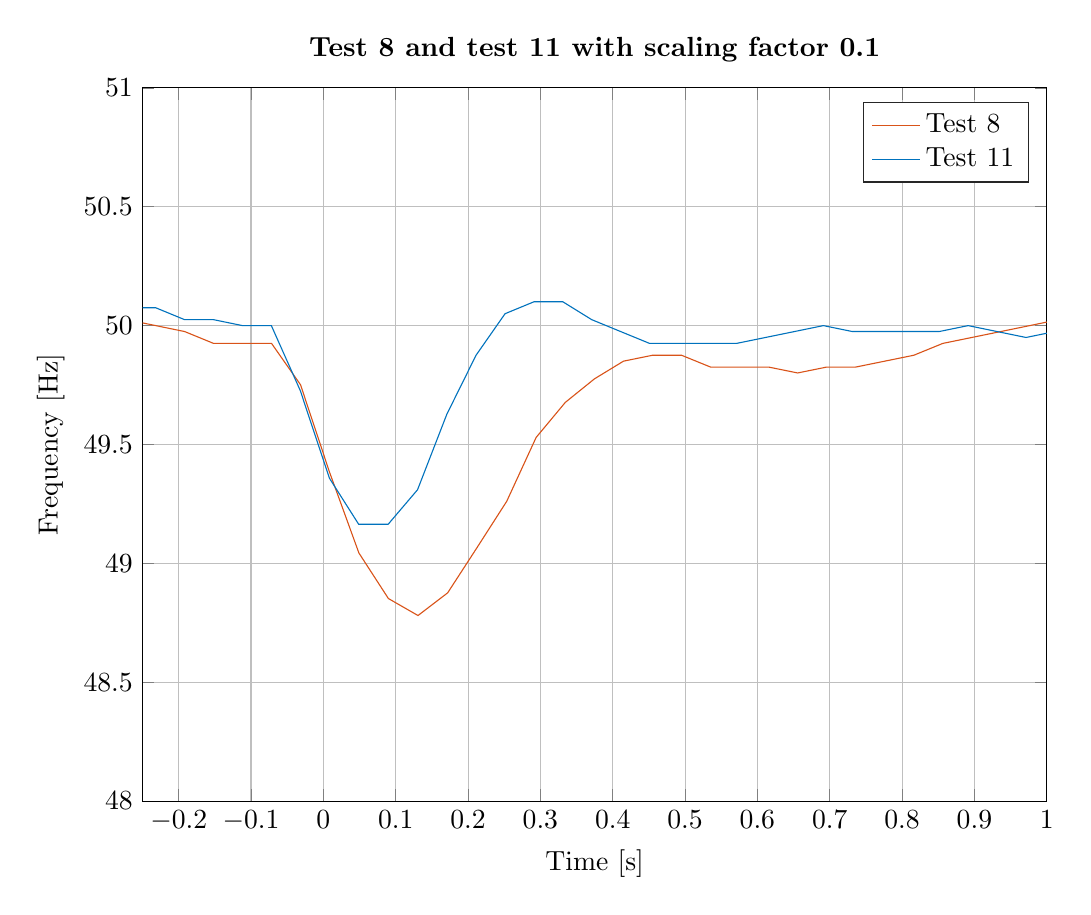
\begin{tikzpicture}

\begin{axis}[%
width=4.521in,
height=3.566in,
at={(0.758in,0.481in)},
scale only axis,
xmin=-0.25,
xmax=1,
xlabel={Time [s]},
xmajorgrids,
ymin=48,
ymax=51,
ylabel={Frequency [Hz]},
ymajorgrids,
axis background/.style={fill=white},
title style={font=\bfseries},
title={Test 8 and test 11 with scaling factor 0.1},
legend style={legend cell align=left,align=left,draw=white!15!black}
]
\addplot [color=mycolor1,solid]
  table[row sep=crcr]{%
-0.271800000000001	50.0250125062532\\
-0.231820000000001	49.9999999999988\\
-0.19182	49.9750124937529\\
-0.1518	49.9251123315044\\
-0.111740000000001	49.9251123315022\\
-0.0716800000000006	49.9251123315022\\
-0.0316200000000002	49.751243781094\\
0.00858000000000025	49.382716049383\\
0.04908	49.0436488474745\\
0.0898599999999998	48.8519785051305\\
0.130799999999999	48.7804878048776\\
0.171799999999999	48.8758553274684\\
0.212719999999999	49.0677134445528\\
0.25348	49.2610837438429\\
0.294079999999999	49.5294700346697\\
0.33446	49.6770988574268\\
0.37472	49.776007964162\\
0.414899999999999	49.850448654038\\
0.455019999999999	49.8753117206974\\
0.49512	49.8753117206996\\
0.535219999999999	49.8256103637258\\
0.57536	49.825610363728\\
0.615499999999999	49.8256103637258\\
0.65564	49.8007968127488\\
0.6958	49.825610363728\\
0.735939999999999	49.825610363728\\
0.776079999999999	49.850448654038\\
0.816199999999998	49.8753117206974\\
0.856299999999999	49.9251123315022\\
0.89636	49.9500499500507\\
0.936399999999999	49.9750124937529\\
0.976419999999999	49.9999999999988\\
1.01642	50.0250125062532\\
};
\addlegendentry{Test 8};

\addplot [color=mycolor2,solid]
  table[row sep=crcr]{%
-0.27176	50.0751126690017\\
-0.231819999999999	50.0751126690062\\
-0.191880000000001	50.0250125062532\\
-0.151900000000001	50.0250125062532\\
-0.111920000000001	49.9999999999966\\
-0.0719199999999987	50.0000000000011\\
-0.0319199999999995	49.7265042267554\\
0.00829999999999842	49.3583415597226\\
0.0488199999999992	49.1642084562416\\
0.089500000000001	49.1642084562459\\
0.130179999999999	49.309664694281\\
0.170739999999999	49.627791563273\\
0.211040000000001	49.8753117206996\\
0.251139999999999	50.0500500500492\\
0.2911	50.1002004008033\\
0.331019999999999	50.1002004007989\\
0.370940000000001	50.0250125062532\\
0.410920000000001	49.9750124937551\\
0.450939999999999	49.9251123315022\\
0.491	49.9251123315022\\
0.53106	49.9251123315022\\
0.571120000000001	49.9251123315022\\
0.611180000000001	49.9500499500529\\
0.651219999999999	49.9750124937507\\
0.691240000000001	50.0000000000011\\
0.73124	49.9750124937507\\
0.771260000000002	49.9750124937551\\
0.81128	49.9750124937551\\
0.851299999999998	49.9750124937507\\
0.89132	50.0000000000011\\
0.931319999999999	49.9750124937507\\
0.971340000000001	49.9500499500529\\
1.01138	49.9750124937507\\
};
\addlegendentry{Test 11};
\end{axis}
\end{tikzpicture}%
\caption{Step from 10 to 20 kW load. }
\label{fig:test8+11freq10to20kwstep}
\end{figure}

\begin{figure}[H]
\centering
% This file was created by matlab2tikz.
%
%The latest updates can be retrieved from
%  http://www.mathworks.com/matlabcentral/fileexchange/22022-matlab2tikz-matlab2tikz
%where you can also make suggestions and rate matlab2tikz.
%
\definecolor{mycolor1}{rgb}{0.00000,0.44700,0.74100}%
\definecolor{mycolor2}{rgb}{0.85000,0.32500,0.09800}%
%
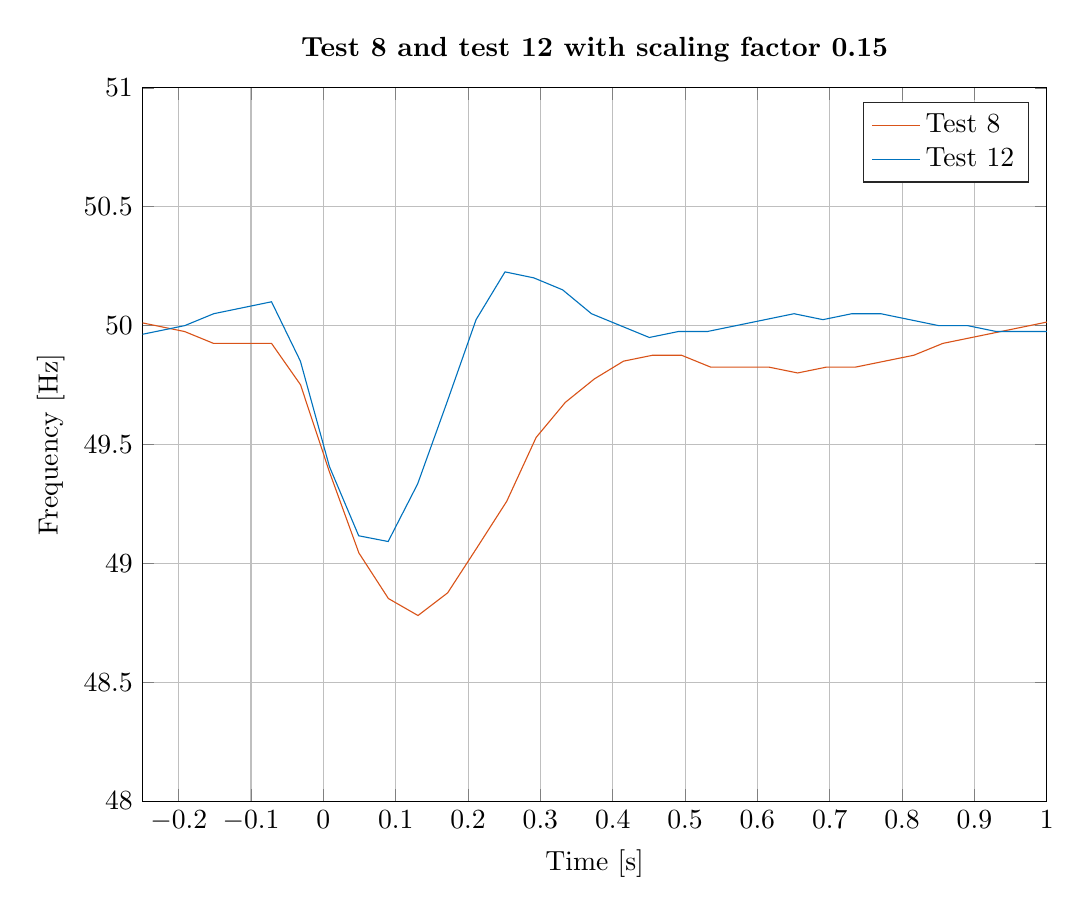
\begin{tikzpicture}

\begin{axis}[%
width=4.521in,
height=3.566in,
at={(0.758in,0.481in)},
scale only axis,
xmin=-0.25,
xmax=1,
xlabel={Time [s]},
xmajorgrids,
ymin=48,
ymax=51,
ylabel={Frequency [Hz]},
ymajorgrids,
axis background/.style={fill=white},
title style={font=\bfseries},
title={Test 8 and test 12 with scaling factor 0.15},
legend style={legend cell align=left,align=left,draw=white!15!black}
]
\addplot [color=mycolor1,solid]
  table[row sep=crcr]{%
-0.271800000000001	50.0250125062532\\
-0.231820000000001	49.9999999999988\\
-0.19182	49.9750124937529\\
-0.1518	49.9251123315044\\
-0.111740000000001	49.9251123315022\\
-0.0716800000000006	49.9251123315022\\
-0.0316200000000002	49.751243781094\\
0.00858000000000025	49.382716049383\\
0.04908	49.0436488474745\\
0.0898599999999998	48.8519785051305\\
0.130799999999999	48.7804878048776\\
0.171799999999999	48.8758553274684\\
0.212719999999999	49.0677134445528\\
0.25348	49.2610837438429\\
0.294079999999999	49.5294700346697\\
0.33446	49.6770988574268\\
0.37472	49.776007964162\\
0.414899999999999	49.850448654038\\
0.455019999999999	49.8753117206974\\
0.49512	49.8753117206996\\
0.535219999999999	49.8256103637258\\
0.57536	49.825610363728\\
0.615499999999999	49.8256103637258\\
0.65564	49.8007968127488\\
0.6958	49.825610363728\\
0.735939999999999	49.825610363728\\
0.776079999999999	49.850448654038\\
0.816199999999998	49.8753117206974\\
0.856299999999999	49.9251123315022\\
0.89636	49.9500499500507\\
0.936399999999999	49.9750124937529\\
0.976419999999999	49.9999999999988\\
1.01642	50.0250125062532\\
};
\addlegendentry{Test 8};

\addplot [color=mycolor2,solid]
  table[row sep=crcr]{%
-0.271660000000001	49.9500499500485\\
-0.231619999999999	49.9750124937551\\
-0.191600000000001	50.0000000000011\\
-0.151600000000002	50.0500500500492\\
-0.111640000000001	50.0751126690017\\
-0.0716999999999999	50.1002004008033\\
-0.0317800000000013	49.8504486540358\\
0.00834000000000046	49.4071146245075\\
0.0488199999999992	49.1159135559918\\
0.0895399999999995	49.0918016691218\\
0.130279999999999	49.3339911198816\\
0.170819999999999	49.6770988574268\\
0.211079999999999	50.0250125062532\\
0.251059999999999	50.2260170768472\\
0.290879999999998	50.2008032128493\\
0.330719999999999	50.150451354062\\
0.3706	50.0500500500492\\
0.41056	50.0000000000011\\
0.450559999999999	49.9500499500485\\
0.490600000000001	49.9750124937551\\
0.530619999999999	49.9750124937507\\
0.570640000000001	50.0000000000011\\
0.61064	50.0250125062532\\
0.65062	50.0500500500492\\
0.690580000000001	50.0250125062532\\
0.730560000000001	50.0500500500537\\
0.770519999999998	50.0500500500492\\
0.810479999999998	50.0250125062532\\
0.850459999999998	49.9999999999966\\
0.890460000000001	50.0000000000011\\
0.93046	49.9750124937551\\
0.970479999999998	49.9750124937507\\
1.0105	49.9750124937551\\
};
\addlegendentry{Test 12};
\end{axis}
\end{tikzpicture}%
\caption{Step from 10 to 20 kW load. }
\label{fig:test8+12freq10to20kwstep}
\end{figure}

\begin{figure}[H]
\centering
% This file was created by matlab2tikz.
%
%The latest updates can be retrieved from
%  http://www.mathworks.com/matlabcentral/fileexchange/22022-matlab2tikz-matlab2tikz
%where you can also make suggestions and rate matlab2tikz.
%
\definecolor{mycolor1}{rgb}{0.00000,0.44700,0.74100}%
\definecolor{mycolor2}{rgb}{0.85000,0.32500,0.09800}%
%
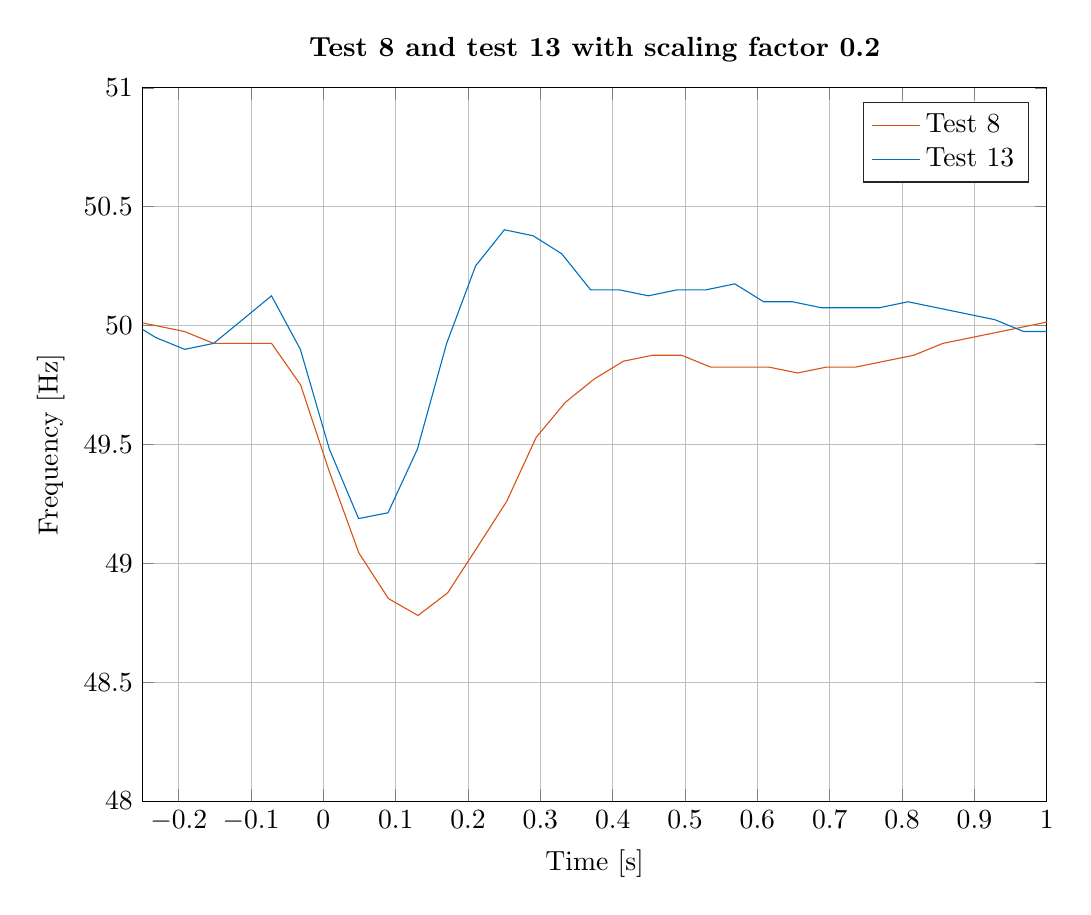
\begin{tikzpicture}

\begin{axis}[%
width=4.521in,
height=3.566in,
at={(0.758in,0.481in)},
scale only axis,
xmin=-0.25,
xmax=1,
xlabel={Time [s]},
xmajorgrids,
ymin=48,
ymax=51,
ylabel={Frequency [Hz]},
ymajorgrids,
axis background/.style={fill=white},
title style={font=\bfseries},
title={Test 8 and test 13 with scaling factor 0.2},
legend style={legend cell align=left,align=left,draw=white!15!black}
]
\addplot [color=mycolor1,solid]
  table[row sep=crcr]{%
-0.271800000000001	50.0250125062532\\
-0.231820000000001	49.9999999999988\\
-0.19182	49.9750124937529\\
-0.1518	49.9251123315044\\
-0.111740000000001	49.9251123315022\\
-0.0716800000000006	49.9251123315022\\
-0.0316200000000002	49.751243781094\\
0.00858000000000025	49.382716049383\\
0.04908	49.0436488474745\\
0.0898599999999998	48.8519785051305\\
0.130799999999999	48.7804878048776\\
0.171799999999999	48.8758553274684\\
0.212719999999999	49.0677134445528\\
0.25348	49.2610837438429\\
0.294079999999999	49.5294700346697\\
0.33446	49.6770988574268\\
0.37472	49.776007964162\\
0.414899999999999	49.850448654038\\
0.455019999999999	49.8753117206974\\
0.49512	49.8753117206996\\
0.535219999999999	49.8256103637258\\
0.57536	49.825610363728\\
0.615499999999999	49.8256103637258\\
0.65564	49.8007968127488\\
0.6958	49.825610363728\\
0.735939999999999	49.825610363728\\
0.776079999999999	49.850448654038\\
0.816199999999998	49.8753117206974\\
0.856299999999999	49.9251123315022\\
0.89636	49.9500499500507\\
0.936399999999999	49.9750124937529\\
0.976419999999999	49.9999999999988\\
1.01642	50.0250125062532\\
};
\addlegendentry{Test 8};

\addplot [color=mycolor2,solid]
  table[row sep=crcr]{%
-0.271880000000003	50.0250125062532\\
-0.231900000000003	49.9500499500485\\
-0.191860000000002	49.9001996007988\\
-0.151780000000002	49.9251123315022\\
-0.111720000000002	50.0250125062532\\
-0.0717400000000019	50.1253132832088\\
-0.0318400000000025	49.9001996007988\\
0.00823999999999714	49.4804552201868\\
0.0486599999999981	49.1883915395978\\
0.0893199999999972	49.2125984251971\\
0.129959999999997	49.4804552201868\\
0.170379999999998	49.9251123315022\\
0.210439999999998	50.2512562814075\\
0.250239999999998	50.4032258064508\\
0.289919999999999	50.3778337531488\\
0.329619999999998	50.3018108651942\\
0.369379999999996	50.150451354062\\
0.409259999999996	50.150451354062\\
0.449139999999996	50.1253132832088\\
0.489039999999996	50.150451354062\\
0.528919999999996	50.150451354062\\
0.568799999999996	50.1756146512784\\
0.608659999999997	50.1002004008033\\
0.648579999999995	50.1002004007989\\
0.688499999999998	50.0751126690062\\
0.728439999999996	50.0751126690017\\
0.768379999999997	50.0751126690017\\
0.808319999999998	50.1002004008033\\
0.848239999999997	50.0751126690017\\
0.888179999999998	50.0500500500537\\
0.928139999999996	50.0250125062532\\
0.968119999999995	49.9750124937507\\
1.00814	49.9750124937551\\
};
\addlegendentry{Test 13};
\end{axis}
\end{tikzpicture}%
\caption{Step from 10 to 20 kW load. }
\label{fig:test8+13freq10to20kwstep}
\end{figure}

\begin{figure}[H]
\centering
% This file was created by matlab2tikz.
%
%The latest updates can be retrieved from
%  http://www.mathworks.com/matlabcentral/fileexchange/22022-matlab2tikz-matlab2tikz
%where you can also make suggestions and rate matlab2tikz.
%
\definecolor{mycolor1}{rgb}{0.00000,0.44700,0.74100}%
\definecolor{mycolor2}{rgb}{0.85000,0.32500,0.09800}%
%
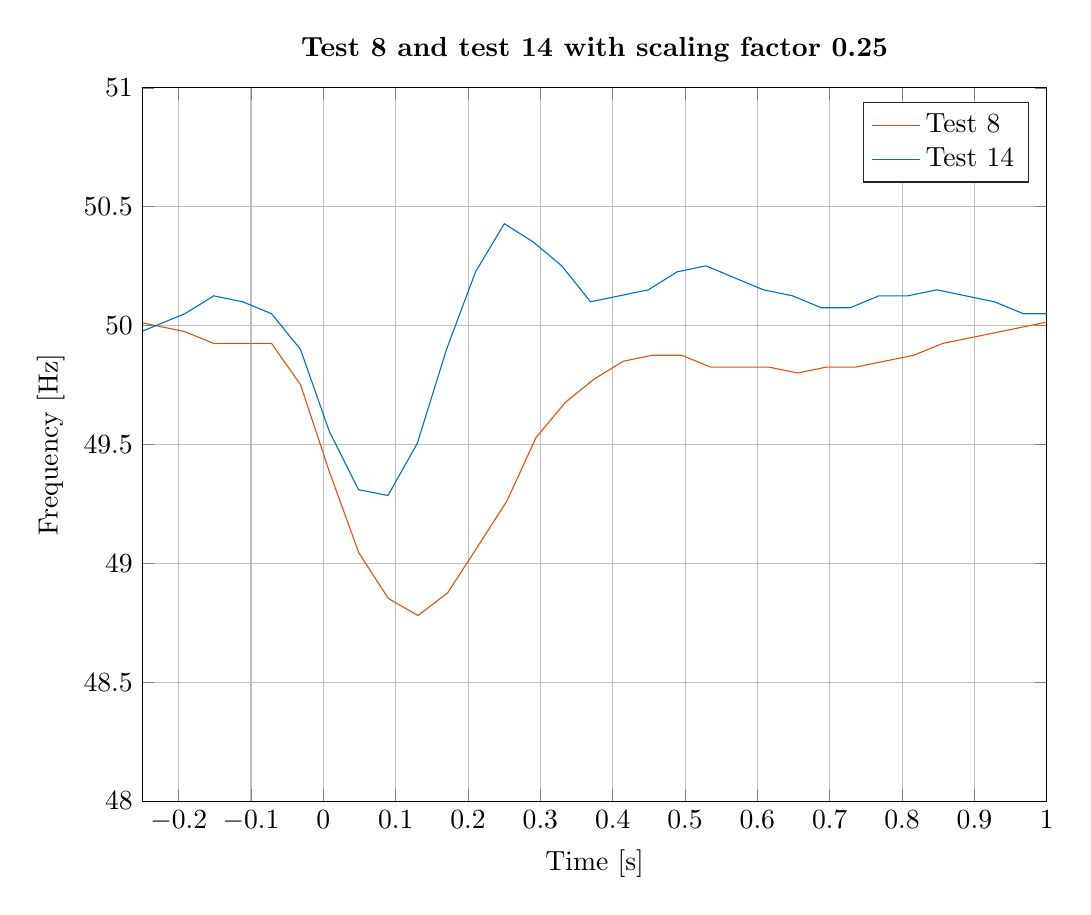
\begin{tikzpicture}

\begin{axis}[%
width=4.521in,
height=3.566in,
at={(0.758in,0.481in)},
scale only axis,
xmin=-0.25,
xmax=1,
xlabel={Time [s]},
xmajorgrids,
ymin=48,
ymax=51,
ylabel={Frequency [Hz]},
ymajorgrids,
axis background/.style={fill=white},
title style={font=\bfseries},
title={Test 8 and test 14 with scaling factor 0.25},
legend style={legend cell align=left,align=left,draw=white!15!black}
]
\addplot [color=mycolor1,solid]
  table[row sep=crcr]{%
-0.271800000000001	50.0250125062532\\
-0.231820000000001	49.9999999999988\\
-0.19182	49.9750124937529\\
-0.1518	49.9251123315044\\
-0.111740000000001	49.9251123315022\\
-0.0716800000000006	49.9251123315022\\
-0.0316200000000002	49.751243781094\\
0.00858000000000025	49.382716049383\\
0.04908	49.0436488474745\\
0.0898599999999998	48.8519785051305\\
0.130799999999999	48.7804878048776\\
0.171799999999999	48.8758553274684\\
0.212719999999999	49.0677134445528\\
0.25348	49.2610837438429\\
0.294079999999999	49.5294700346697\\
0.33446	49.6770988574268\\
0.37472	49.776007964162\\
0.414899999999999	49.850448654038\\
0.455019999999999	49.8753117206974\\
0.49512	49.8753117206996\\
0.535219999999999	49.8256103637258\\
0.57536	49.825610363728\\
0.615499999999999	49.8256103637258\\
0.65564	49.8007968127488\\
0.6958	49.825610363728\\
0.735939999999999	49.825610363728\\
0.776079999999999	49.850448654038\\
0.816199999999998	49.8753117206974\\
0.856299999999999	49.9251123315022\\
0.89636	49.9500499500507\\
0.936399999999999	49.9750124937529\\
0.976419999999999	49.9999999999988\\
1.01642	50.0250125062532\\
};
\addlegendentry{Test 8};

\addplot [color=mycolor2,solid]
  table[row sep=crcr]{%
-0.271520000000002	49.9500499500485\\
-0.231480000000001	50.0000000000011\\
-0.191480000000002	50.0500500500492\\
-0.151520000000001	50.1253132832088\\
-0.111620000000002	50.1002004008033\\
-0.0717000000000034	50.0500500500492\\
-0.0317400000000028	49.9001996007988\\
0.00833999999999691	49.5540138751242\\
0.0486999999999966	49.309664694281\\
0.0892599999999959	49.28536224741\\
0.129839999999998	49.5049504950517\\
0.170239999999996	49.9001996007988\\
0.210319999999996	50.2260170768428\\
0.250139999999998	50.4286434694935\\
0.289799999999996	50.3524672708929\\
0.329519999999999	50.2512562814075\\
0.369319999999998	50.1002004008033\\
0.409239999999997	50.1253132832088\\
0.449139999999996	50.150451354062\\
0.489019999999996	50.2260170768428\\
0.528839999999999	50.2512562814075\\
0.568639999999998	50.2008032128538\\
0.608479999999997	50.150451354062\\
0.648359999999997	50.1253132832088\\
0.688259999999996	50.0751126690017\\
0.728199999999998	50.0751126690017\\
0.768139999999999	50.1253132832088\\
0.808039999999998	50.1253132832088\\
0.847939999999998	50.150451354062\\
0.887819999999998	50.1253132832088\\
0.927719999999997	50.1002004008033\\
0.967639999999996	50.0500500500492\\
1.0076	50.0500500500492\\
};
\addlegendentry{Test 14};
\end{axis}
\end{tikzpicture}%
\caption{Step from 10 to 20 kW load. }
\label{fig:test8+14freq10to20kwstep}
\end{figure}

%The two first test shown below has the characteristic as mention, but the last two has large overshoot and reach steady state around the same time as the uncontrolled signal. 
The tests shows clearly that the drop in frequency, when a step is applied, is improved and for lower values of the scaling factor the settling time has also improved. For larger values of the scaling factor overshoot is getting more pronounced and the same characteristic shown on \figref{fig:modelfreq_volt} is appearing. This disturbance is unwanted thus making the test performed with a scaling factor of 0.1 the most ideal for comparison with the reference measurements.  Therefore further comparisons will be done between controller with scaling factor 0.1 and reference measurement.

%These test has a scaling factor of 0.2 and 0.25 and are deemed not successful at this load size. \figref{fig:test8+11freq10to20kwstep} and \figref{fig:test8+12freq10to20kwstep} has a scaling factor of 0.1 and 0.15 and for this load size these are the best fit. Especially \figref{fig:test8+11freq10to20kwstep} takes a small fall in frequency and has a small overshoot. Therefore figures with a scaling factor of 0.1 will be shown, rest can be found on the CD \fxnote{Need to put plots on the cd and make a reference here}.   

%A variety of different steps have been applied to the genset to see how it reacts with the controller. 
 On \figref{fig:test8+11freq-1020-4050-1030-1050} it is shown how the frequency reacts to different steps in loads. 
 %The first figure shows a step in load from 10-30 kW. It can be seen that the controlled signal takes a small fall in frequency and react faster to the change in load at the cost of an overshoot. But the controlled signal reach steady state before the base measurement approximately 0.5 seconds. The second figure shows a step in load from 10-50 kW. At this step size the controlled signal reacts faster but it takes more time for it to reach steady state. A reason to why it does not go back to the reference value 50 Hz could be that the voltage is to high(higher than the reference) and therefore the controller is trying to decrease it by decreasing the frequency, this will be analyzed further when the voltage measurement are shown. The third figure shows a step from 40-50 kW in load. It also react faster to a change in load but reach steady state around the same time as the base measurement.      


\begin{figure}[H]
\centering
% This file was created by matlab2tikz.
%
%The latest updates can be retrieved from
%  http://www.mathworks.com/matlabcentral/fileexchange/22022-matlab2tikz-matlab2tikz
%where you can also make suggestions and rate matlab2tikz.
%
\definecolor{mycolor1}{rgb}{0.85000,0.32500,0.09800}%
\definecolor{mycolor2}{rgb}{0.00000,0.44700,0.74100}%
%
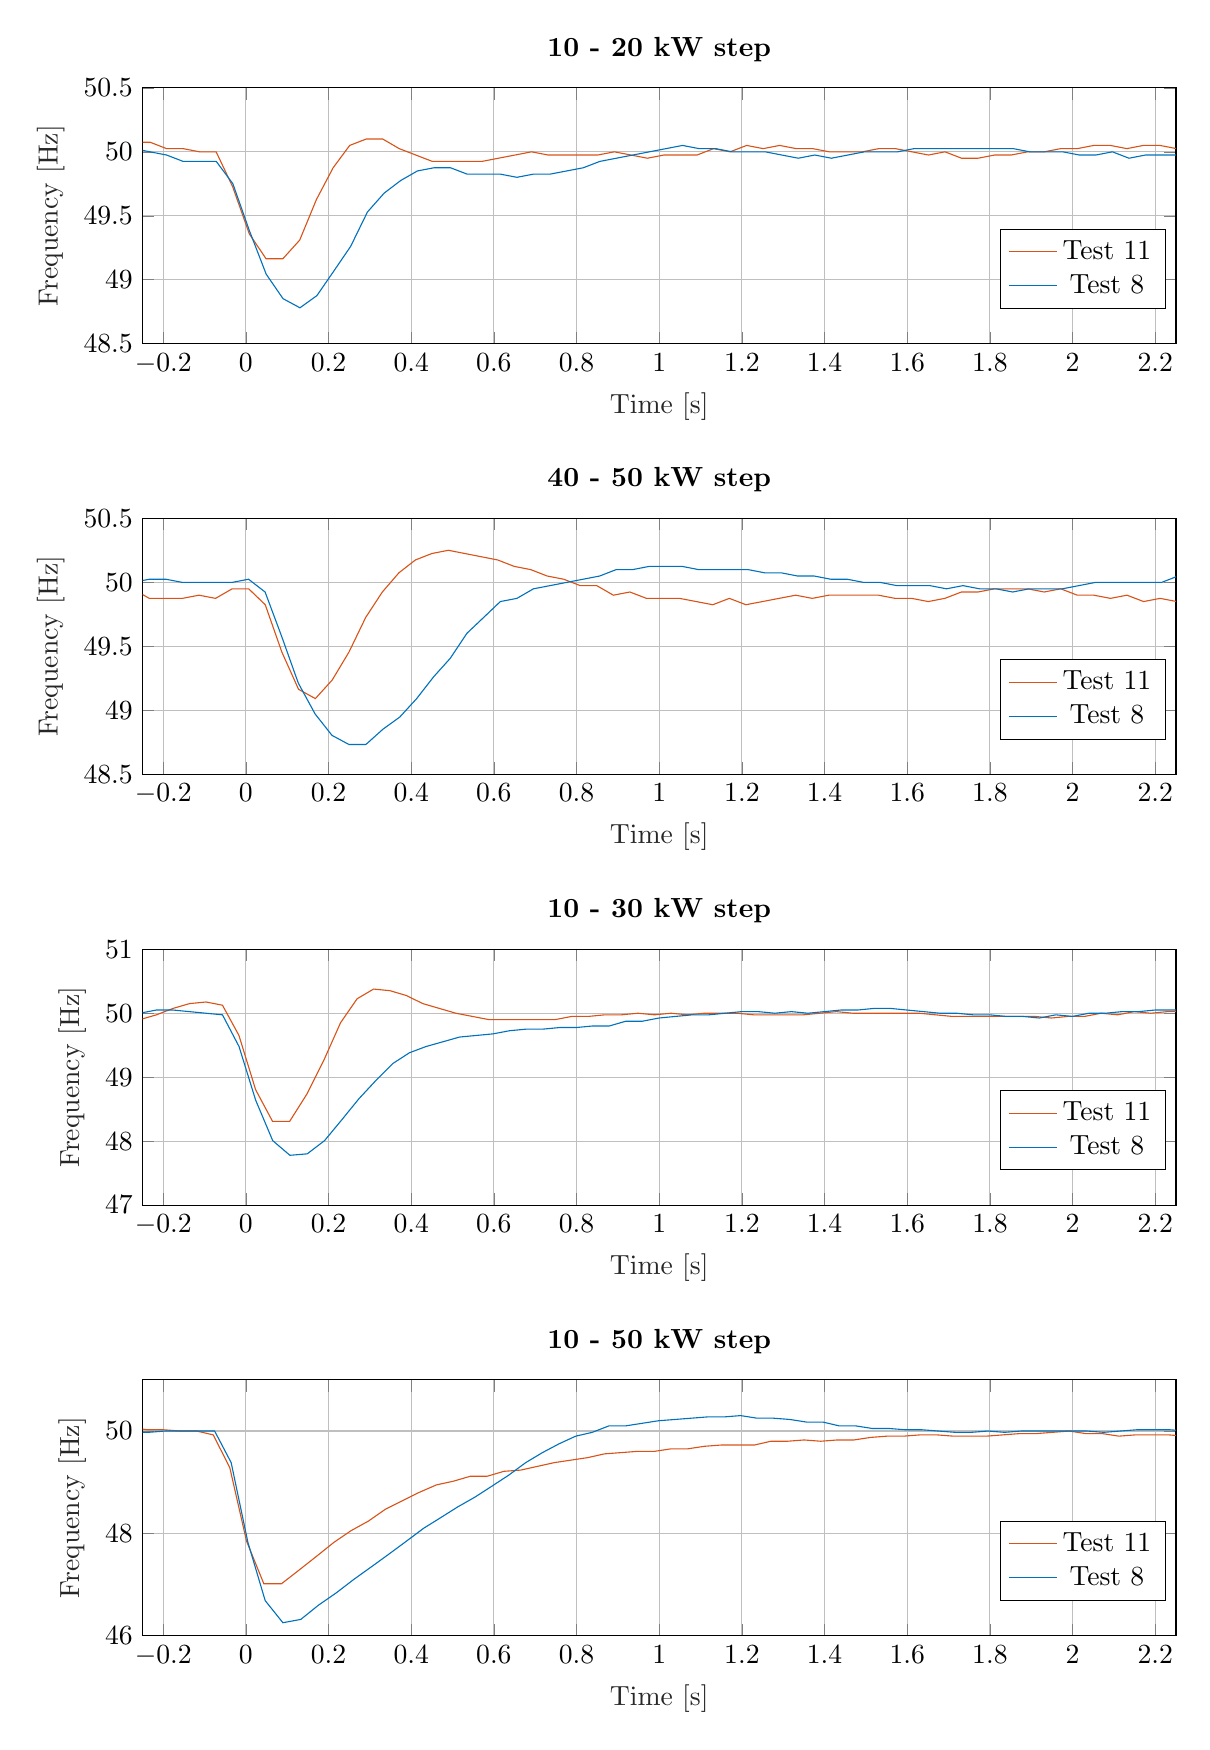
\begin{tikzpicture}

\begin{axis}[%
width=5.167in,
height=1.279in,
at={(0.867in,7.534in)},
%at={(1.297in,7.931in)},
scale only axis,
xmin=-0.25,
xmax=2.25,
xlabel style={font=\color{white!15!black}},
xlabel={Time [s]},
ymin=48.5,
ymax=50.5,
ylabel style={font=\color{white!15!black}},
ylabel={Frequency [Hz]},
axis background/.style={fill=white},
title style={font=\bfseries},
title={10 - 20 kW step},
%axis x line*=bottom,
%axis y line*=left
xmajorgrids,
ymajorgrids,
legend style={at={(0.99,0.45)},anchor=north east}
]
\addplot [color=mycolor1, solid]
  table[row sep=crcr]{%
-0.27176	50.0751126690017\\
-0.231819999999999	50.0751126690062\\
-0.191880000000005	50.0250125062532\\
-0.151900000000005	50.0250125062532\\
-0.111920000000005	49.9999999999966\\
-0.0719199999999987	50.0000000000011\\
-0.0319199999999995	49.7265042267554\\
0.00829999999999842	49.3583415597226\\
0.0488199999999992	49.1642084562416\\
0.089500000000001	49.1642084562459\\
0.130180000000003	49.309664694281\\
0.170740000000002	49.627791563273\\
0.211040000000004	49.8753117206996\\
0.251139999999999	50.0500500500492\\
0.2911	50.1002004008033\\
0.331020000000002	50.1002004007989\\
0.370940000000004	50.0250125062532\\
0.450940000000003	49.9251123315022\\
0.571120000000001	49.9251123315022\\
0.691240000000001	50.0000000000011\\
0.73124	49.9750124937507\\
0.851300000000002	49.9750124937507\\
0.89132	50.0000000000011\\
0.971340000000005	49.9500499500529\\
1.01138	49.9750124937507\\
1.09142	49.9750124937507\\
1.13144	50.0250125062532\\
1.17142	50.0000000000011\\
1.21142	50.0500500500492\\
1.25138	50.0250125062532\\
1.29136	50.0500500500492\\
1.33132000000001	50.0250125062532\\
1.37130000000001	50.0250125062532\\
1.41128000000001	50.0000000000011\\
1.49128	50.0000000000011\\
1.53128	50.0250125062532\\
1.57126	50.0250125062532\\
1.65124	49.9750124937551\\
1.69126	50.0000000000011\\
1.73126	49.9500499500485\\
1.7713	49.9500499500485\\
1.81134	49.9750124937551\\
1.85136	49.9750124937507\\
1.89138000000001	50.0000000000011\\
1.93138	50.0000000000011\\
1.97138	50.0250125062532\\
2.01136	50.0250125062532\\
2.05134	50.0500500500492\\
2.0913	50.0500500500492\\
2.13126	50.0250125062532\\
2.17124	50.0500500500492\\
2.21120000000001	50.0500500500537\\
2.25116	50.0250125062532\\
};
\addlegendentry{Test 11}

\addplot [color=mycolor2, solid]
  table[row sep=crcr]{%
-0.271799999999999	50.0250125062532\\
-0.19182	49.9750124937529\\
-0.151800000000001	49.9251123315044\\
-0.0716800000000006	49.9251123315022\\
-0.0316200000000038	49.751243781094\\
0.00858000000000203	49.382716049383\\
0.0490800000000036	49.0436488474745\\
0.0898600000000016	48.8519785051305\\
0.130800000000001	48.7804878048776\\
0.171799999999998	48.8758553274684\\
0.212719999999997	49.0677134445528\\
0.253480000000003	49.2610837438429\\
0.294080000000001	49.5294700346697\\
0.33446	49.6770988574268\\
0.374720000000003	49.776007964162\\
0.414900000000003	49.850448654038\\
0.455019999999998	49.8753117206974\\
0.49512	49.8753117206996\\
0.535220000000002	49.8256103637258\\
0.615499999999997	49.8256103637258\\
0.655639999999998	49.8007968127488\\
0.695799999999998	49.825610363728\\
0.735939999999999	49.825610363728\\
0.816200000000002	49.8753117206974\\
0.856299999999997	49.9251123315022\\
1.0564	50.0500500500514\\
1.09636	50.0250125062532\\
1.13634	50.0250125062532\\
1.17632	49.9999999999988\\
1.25632	49.9999999999988\\
1.33634	49.9500499500507\\
1.37638	49.9750124937529\\
1.4164	49.9500499500507\\
1.49646	49.9999999999988\\
1.57646	49.9999999999988\\
1.61646	50.0250125062532\\
1.85634	50.0250125062532\\
1.89632	50.0000000000011\\
1.97632	50.0000000000011\\
2.01632	49.9750124937529\\
2.05634	49.9750124937529\\
2.09636	49.9999999999988\\
2.13636	49.9500499500507\\
2.1764	49.9750124937529\\
2.25644	49.9750124937529\\
};
\addlegendentry{Test 8}

\end{axis}

\begin{axis}[%
width=5.167in,
height=1.279in,
at={(0.867in,5.381in)},
%at={(1.297in,5.661in)},
scale only axis,
xmin=-0.25,
xmax=2.25,
xlabel style={font=\color{white!15!black}},
xlabel={Time [s]},
ymin=48.5,
ymax=50.5,
ylabel style={font=\color{white!15!black}},
ylabel={Frequency [Hz]},
axis background/.style={fill=white},
title style={font=\bfseries},
title={40 - 50 kW step},
%axis x line*=bottom,
%axis y line*=left
xmajorgrids,
ymajorgrids,
legend style={at={(0.99,0.45)},anchor=north east}
]
\addplot [color=mycolor1, solid]
  table[row sep=crcr]{%
-0.273780000000016	49.950049950044\\
-0.233740000000012	49.875311720704\\
-0.153540000000021	49.8753117206863\\
-0.113440000000011	49.9001996008121\\
-0.0733600000000223	49.8753117206863\\
-0.0332600000000127	49.9500499500618\\
0.0067799999999778	49.950049950044\\
0.0468199999999825	49.825610363717\\
0.0869599999999906	49.4559841740978\\
0.12739999999998	49.1642084562331\\
0.168079999999989	49.0918016691218\\
0.208819999999989	49.2368291482151\\
0.249439999999979	49.4559841740804\\
0.289879999999982	49.7265042267466\\
0.330099999999987	49.9251123315066\\
0.370159999999984	50.0751126690017\\
0.410099999999986	50.1756146512739\\
0.44995999999999	50.2260170768562\\
0.489779999999982	50.2512562814075\\
0.609239999999986	50.1756146512739\\
0.64909999999999	50.1253132832222\\
0.688999999999979	50.10020040079\\
0.728919999999988	50.0500500500581\\
0.768879999999982	50.0250125062532\\
0.808859999999981	49.9750124937551\\
0.84887999999998	49.9750124937551\\
0.888899999999978	49.9001996007944\\
0.928979999999981	49.9251123315066\\
0.969039999999978	49.8753117206863\\
1.04923999999998	49.875311720704\\
1.12945999999998	49.825610363717\\
1.16959999999999	49.875311720704\\
1.20969999999998	49.8256103637346\\
1.33005999999999	49.9001996008121\\
1.37013999999998	49.8753117206863\\
1.41023999999999	49.9001996007944\\
1.53047999999998	49.9001996007944\\
1.57055999999999	49.875311720704\\
1.61065999999998	49.8753117206863\\
1.65075999999999	49.8504486540534\\
1.69087999999998	49.8753117206863\\
1.73097999999999	49.9251123315066\\
1.77103999999999	49.9251123315066\\
1.81109999999998	49.950049950044\\
1.89117999999998	49.950049950044\\
1.93121999999998	49.9251123315066\\
1.97127999999998	49.950049950044\\
2.01131999999998	49.9001996007944\\
2.05139999999999	49.9001996007944\\
2.09147999999999	49.875311720704\\
2.13157999999999	49.9001996007944\\
2.17165999999999	49.8504486540358\\
2.21177999999999	49.875311720704\\
2.25187999999999	49.8504486540358\\
};
\addlegendentry{Test 11}

\addplot [color=mycolor2, solid]
  table[row sep=crcr]{%
-0.273499999999999	50.0000000000011\\
-0.233499999999999	50.0250125062532\\
-0.193519999999999	50.0250125062532\\
-0.15354	50.0000000000011\\
-0.11354	50.0000000000011\\
-0.0735400000000013	50.0000000000011\\
-0.0335400000000021	50.0000000000011\\
0.00645999999999702	50.0250125062532\\
0.0464399999999969	49.9251123314978\\
0.0865000000000009	49.5785820525527\\
0.126840000000001	49.2125984252014\\
0.167479999999998	48.9715964740416\\
0.208320000000001	48.8042947779433\\
0.249299999999998	48.7329434697827\\
0.29034	48.7329434697912\\
0.331379999999996	48.8519785051221\\
0.372320000000002	48.947626040143\\
0.413179999999997	49.0918016691218\\
0.453919999999997	49.2610837438365\\
0.494520000000001	49.4071146245118\\
0.534999999999997	49.6031746031731\\
0.575319999999998	49.7265042267554\\
0.615539999999996	49.8504486540358\\
0.655659999999997	49.8753117206952\\
0.69576	49.9500499500529\\
0.735799999999998	49.9750124937551\\
0.775819999999996	49.9999999999922\\
0.815820000000002	50.0250125062532\\
0.855800000000002	50.0500500500581\\
0.895759999999996	50.1002004007989\\
0.935679999999998	50.1002004007989\\
0.9756	50.1253132832133\\
1.0155	50.1253132832043\\
1.0554	50.1253132832043\\
1.0953	50.1002004008078\\
1.13522	50.1002004007989\\
1.21506	50.1002004008078\\
1.25498	50.0751126690017\\
1.29492	50.0751126690017\\
1.33486	50.0500500500492\\
1.37482	50.0500500500492\\
1.41478	50.0250125062532\\
1.45476	50.0250125062532\\
1.49474	50.0000000000011\\
1.53474	50.0000000000011\\
1.57474	49.9750124937551\\
1.61476	49.9750124937463\\
1.65478	49.9750124937551\\
1.6948	49.9500499500529\\
1.73484	49.9750124937551\\
1.77486	49.950049950044\\
1.8149	49.9500499500529\\
1.85494	49.9251123315066\\
1.895	49.950049950044\\
1.93504	49.9500499500529\\
1.97508	49.9500499500529\\
2.01512	49.9750124937463\\
2.05514	50.0000000000011\\
2.09514	50.0000000000011\\
2.13514	50.0000000000011\\
2.17514	50.0000000000011\\
2.21514	50.0000000000011\\
2.25514	50.0500500500492\\
};
\addlegendentry{Test 8}

\end{axis}

\begin{axis}[%
width=5.167in,
height=1.279in,
at={(0.867in,3.227in)},
%at={(1.297in,3.391in)},
scale only axis,
xmin=-0.25,
xmax=2.25,
xlabel style={font=\color{white!15!black}},
xlabel={Time [s]},
ymin=47,
ymax=51,
ylabel style={font=\color{white!15!black}},
ylabel={Frequency [Hz]},
axis background/.style={fill=white},
title style={font=\bfseries},
title={10 - 30 kW step},
%axis x line*=bottom,
%axis y line*=left
xmajorgrids,
ymajorgrids,
legend style={at={(0.99,0.45)},anchor=north east}
]
\addplot [color=mycolor1, solid]
  table[row sep=crcr]{%
-0.256440000000026	49.9001996007944\\
-0.216360000000023	49.9750124937551\\
-0.176340000000025	50.0751126690017\\
-0.136400000000023	50.1504513540665\\
-0.0965200000000266	50.1756146512739\\
-0.0566600000000221	50.1253132832043\\
-0.0167600000000192	49.6524329692209\\
0.0235199999999764	48.8042947779349\\
0.0644999999999811	48.3091787439662\\
0.105899999999977	48.3091787439662\\
0.147299999999973	48.7329434697743\\
0.188339999999982	49.2610837438451\\
0.22893999999998	49.8504486540358\\
0.269059999999982	50.2260170768562\\
0.308879999999974	50.3778337531353\\
0.348579999999984	50.3524672708929\\
0.388299999999987	50.2765208647647\\
0.42807999999998	50.1504513540665\\
0.507899999999978	49.9999999999922\\
0.587939999999975	49.9001996007944\\
0.748259999999974	49.9001996007944\\
0.788339999999977	49.950049950044\\
0.828379999999981	49.950049950044\\
0.868419999999986	49.9750124937551\\
0.908439999999985	49.9750124937551\\
0.948459999999983	50.0000000000099\\
0.988459999999975	49.9750124937551\\
1.02847999999997	49.9999999999922\\
1.06847999999998	49.9750124937551\\
1.10849999999998	49.9999999999922\\
1.18849999999998	49.9999999999922\\
1.22849999999998	49.9750124937551\\
1.34855999999998	49.9750124937551\\
1.42857999999998	50.0250125062532\\
1.46855999999998	50.0000000000099\\
1.62855999999998	49.9999999999922\\
1.70857999999998	49.9500499500618\\
1.90877999999998	49.950049950044\\
1.94881999999998	49.9251123315066\\
1.98887999999998	49.950049950044\\
2.02891999999999	49.9500499500618\\
2.06895999999998	49.9999999999922\\
2.10895999999998	49.9750124937551\\
2.14897999999998	50.0250125062532\\
2.18895999999998	49.9999999999922\\
2.22895999999999	50.0250125062532\\
2.26893999999999	50.0250125062532\\
};
\addlegendentry{Test 11}

\addplot [color=mycolor2, solid]
  table[row sep=crcr]{%
-0.256560000000015	50.0000000000011\\
-0.216560000000015	50.0500500500492\\
-0.176600000000015	50.0500500500492\\
-0.136640000000014	50.0250125062532\\
-0.0966600000000142	50.0000000000011\\
-0.056660000000015	49.9750124937463\\
-0.0166400000000095	49.4804552201911\\
0.0237799999999879	48.6381322957206\\
0.0648999999999873	48.0076812289963\\
0.106559999999988	47.7783086478741\\
0.148419999999987	47.8011472275328\\
0.190259999999988	48.0076812289963\\
0.231919999999988	48.3325277912074\\
0.273299999999985	48.6618004866178\\
0.314399999999985	48.9476260401345\\
0.355259999999987	49.2125984251928\\
0.39589999999999	49.3827160493895\\
0.436399999999985	49.4804552201824\\
0.476819999999989	49.5540138751242\\
0.517179999999989	49.6277915632817\\
0.557479999999984	49.6524329692121\\
0.597759999999987	49.6770988574224\\
0.63801999999999	49.7265042267554\\
0.678239999999988	49.7512437810962\\
0.718439999999987	49.7512437810962\\
0.758639999999986	49.776007964162\\
0.798819999999985	49.776007964162\\
0.838999999999984	49.8007968127488\\
0.879159999999985	49.8007968127488\\
0.919319999999985	49.8753117206952\\
0.959419999999987	49.8753117206952\\
0.99951999999999	49.9251123315066\\
1.03957999999999	49.9500499500529\\
1.07961999999998	49.9750124937463\\
1.11963999999999	49.9750124937551\\
1.15965999999999	50.0000000000011\\
1.19965999999999	50.0250125062532\\
1.23963999999999	50.0250125062532\\
1.27961999999999	49.9999999999922\\
1.31961999999999	50.025012506271\\
1.35959999999998	49.9999999999922\\
1.39959999999999	50.0250125062532\\
1.43957999999999	50.0500500500403\\
1.47953999999999	50.0500500500581\\
1.51949999999999	50.0751126690017\\
1.55943999999999	50.0751126690017\\
1.59937999999999	50.0500500500581\\
1.63933999999998	50.0250125062355\\
1.67932	50.0000000000099\\
1.71931999999999	50.0000000000099\\
1.75931999999998	49.9750124937551\\
1.79933999999998	49.9750124937551\\
1.83935999999998	49.950049950044\\
1.87939999999998	49.950049950044\\
1.91943999999999	49.9251123315066\\
1.95949999999998	49.9750124937374\\
1.99952	49.9500499500618\\
2.03955999999999	49.9999999999922\\
2.07955999999999	50.0000000000099\\
2.11955999999999	50.0250125062532\\
2.15953999999999	50.0250125062532\\
2.19951999999999	50.0500500500403\\
2.23947999999999	50.0500500500581\\
2.27943999999999	50.0500500500581\\
};
\addlegendentry{Test 8}

\end{axis}

\begin{axis}[%
width=5.167in,
height=1.279in,
%at={(1.297in,1.122in)},
at={(0.867in,1.074in)},
scale only axis,
xmin=-0.25,
xmax=2.25,
xlabel style={font=\color{white!15!black}},
xlabel={Time [s]},
ymin=46,
ymax=51,
ylabel style={font=\color{white!15!black}},
ylabel={Frequency [Hz]},
axis background/.style={fill=white},
title style={font=\bfseries},
title={10 - 50 kW step},
%axis x line*=bottom,
%axis y line*=left
xmajorgrids,
ymajorgrids,
legend style={at={(0.99,0.45)},anchor=north east}
]
\addplot [color=mycolor1, solid]
  table[row sep=crcr]{%
-0.278920000000028	50.0751126690017\\
-0.238980000000026	50.025012506271\\
-0.199000000000041	50.0250125062355\\
-0.159020000000027	50.0000000000099\\
-0.119020000000035	50.0000000000099\\
-0.0790200000000425	49.9251123314889\\
-0.0389600000000314	49.2853622474057\\
0.0016199999999742	47.8468899521589\\
0.0434199999999692	47.0145745180979\\
0.0859599999999716	47.0145745180979\\
0.128499999999974	47.2813238770874\\
0.170799999999957	47.5511174512368\\
0.212859999999978	47.8240076518397\\
0.254679999999979	48.0538202787183\\
0.296299999999974	48.2392667631444\\
0.337759999999975	48.4730974309328\\
0.420139999999975	48.8042947779518\\
0.461119999999966	48.947626040126\\
0.501979999999975	49.0196078431491\\
0.542779999999965	49.1159135560003\\
0.583499999999958	49.1159135559661\\
0.62421999999998	49.2125984252014\\
0.664859999999976	49.2368291482151\\
0.746039999999965	49.3827160493722\\
0.82699999999997	49.4804552202085\\
0.867419999999953	49.554013875098\\
0.94811999999996	49.6031746031643\\
0.988439999999969	49.6031746031643\\
1.02875999999998	49.6524329692209\\
1.06903999999997	49.6524329692209\\
1.10931999999997	49.7017892643995\\
1.14955999999998	49.7265042267818\\
1.22999999999996	49.7265042267466\\
1.27021999999997	49.8007968127311\\
1.31037999999998	49.8007968127664\\
1.35053999999997	49.825610363717\\
1.39067999999997	49.8007968127664\\
1.43083999999996	49.825610363717\\
1.47097999999997	49.825610363717\\
1.51111999999998	49.875311720704\\
1.55121999999997	49.9001996008121\\
1.59129999999996	49.9001996007767\\
1.63137999999998	49.9251123315244\\
1.67143999999996	49.9251123314889\\
1.71149999999997	49.9001996008121\\
1.79165999999998	49.9001996008121\\
1.87179999999998	49.9500499500795\\
1.91183999999996	49.950049950044\\
1.99189999999996	49.9999999999744\\
2.03189999999998	49.9500499500795\\
2.07193999999996	49.950049950044\\
2.11197999999996	49.9001996007767\\
2.15205999999998	49.9251123315244\\
2.23217999999997	49.9251123314889\\
2.27223999999998	49.9001996008121\\
};
\addlegendentry{Test 11}

\addplot [color=mycolor2, solid]
  table[row sep=crcr]{%
-0.275660000000016	49.9750124937551\\
-0.235640000000018	49.9750124937551\\
-0.195620000000019	49.9999999999922\\
-0.155620000000013	50.0000000000099\\
-0.115620000000021	49.9999999999922\\
-0.0756200000000149	50.0000000000099\\
-0.0356200000000229	49.3827160493722\\
0.00487999999998578	47.8240076518397\\
0.0466999999999871	46.6853408029898\\
0.0895399999999853	46.2534690101787\\
0.132779999999983	46.3177396942958\\
0.175959999999989	46.5983224603967\\
0.218879999999984	46.8384074941491\\
0.261579999999981	47.10315591144\\
0.304039999999986	47.3484848484933\\
0.346279999999979	47.5963826749077\\
0.388299999999987	47.8468899521589\\
0.430099999999982	48.1000481000525\\
0.471679999999978	48.3091787439496\\
0.513079999999988	48.5201358563856\\
0.554299999999984	48.7092060399396\\
0.595359999999985	48.9236790606637\\
0.636239999999987	49.1400491400479\\
0.676939999999988	49.3827160493895\\
0.717439999999982	49.5785820525527\\
0.757779999999983	49.7512437810962\\
0.797979999999981	49.9001996007944\\
0.838059999999984	49.9750124937551\\
0.878079999999983	50.1002004008078\\
0.917999999999978	50.10020040079\\
0.957919999999987	50.1504513540665\\
0.997799999999984	50.2008032128538\\
1.03763999999998	50.2260170768383\\
1.07745999999999	50.2512562814075\\
1.11725999999999	50.2765208647647\\
1.15703999999998	50.2765208647467\\
1.19681999999999	50.3018108651897\\
1.23657999999999	50.2512562814255\\
1.27637999999997	50.2512562813896\\
1.31617999999999	50.2260170768562\\
1.35599999999998	50.1756146512739\\
1.39585999999998	50.1756146512739\\
1.43571999999999	50.1002004008078\\
1.47563999999998	50.1002004008078\\
1.51555999999998	50.0500500500403\\
1.55551999999999	50.0500500500581\\
1.59547999999998	50.0250125062532\\
1.63545999999998	50.0250125062532\\
1.67543999999998	49.9999999999922\\
1.71543999999999	49.9750124937551\\
1.75545999999999	49.9750124937551\\
1.79547999999998	50.0000000000099\\
1.83547999999998	49.9750124937551\\
1.87549999999997	49.9999999999922\\
1.95549999999999	50.0000000000099\\
1.99549999999998	49.9999999999922\\
2.03549999999998	49.9999999999922\\
2.07549999999999	49.9750124937551\\
2.11551999999999	50.0000000000099\\
2.15551999999998	50.0250125062532\\
2.19549999999998	50.0250125062532\\
2.23547999999998	50.0250125062532\\
2.27545999999998	49.9999999999922\\
};
\addlegendentry{Test 8}

\end{axis}
\end{tikzpicture}%
\caption{Frequency disturbance due to various changes in load without and with controller and a scaling factor of 0.1.}
\label{fig:test8+11freq-1020-4050-1030-1050}
\end{figure}

Common for all the steps shown on \figref{fig:test8+11freq-1020-4050-1030-1050} is that the droop in frequency is reduced and for some cases the settling time has improved or stayed the same. Some amount of overshoot is also occurring at lower loads. This means more fuel is consumed to correct the disturbance in the frequency than necessary as overshoot is not wanted. It also means that either the controller is reacting to slow or not enough fuel was injected in to the engine for it to negate the droop in frequency.

%Due to the inlinearities of the genset then the same 10 kW step at different loads will result in different reactions. This could be a result of the diesel engine not being able to provide instant power but is limited to provide energy to the shaft driving the generator an amount of times per round equal to the amount of cylinders in the engine. Furthermore to compensate at larger loads more fuel is needed and the fly   

From the frequency measurements it can be concluded that the system is able to react correct the disturbance in frequency faster when a change in load occurs. Furthermore improved steady state time at steps at lower loads is achieved.  
%and at some load sizes it also reach steady state before the base measurements. 

On \figref{fig:test8+11volt-1020-4050-1030-1050} the Voltage disturbance at various step sizes is shown.

 %it is illustrated how the voltage react to different steps in load with the same scaling factor of 0.1. From the first figure minor changes can be seen in the response. The controlled signal react slightly faster than the base measurement. The time it takes for both to reach steady state is approximately the same. It can also be seen on the controlled signal that the second order characteristic that the controller have been designed from is visible from the response. Which can be said for all four measurements. To conclude on why the frequency from before did not go back to it reference value the third figure will be analyzed. It can be seen when it has reach steady state that it fluctuates around 230 volt, which could be the reason for, that the frequency does not reach 50 Hz because it is trying to decrease the voltage when it goes higher than 230 volt.  



\begin{figure}[H]
\centering
% This file was created by matlab2tikz.
%
%The latest updates can be retrieved from
%  http://www.mathworks.com/matlabcentral/fileexchange/22022-matlab2tikz-matlab2tikz
%where you can also make suggestions and rate matlab2tikz.
%
\definecolor{mycolor1}{rgb}{0.85000,0.32500,0.09800}%
\definecolor{mycolor2}{rgb}{0.00000,0.44700,0.74100}%
%
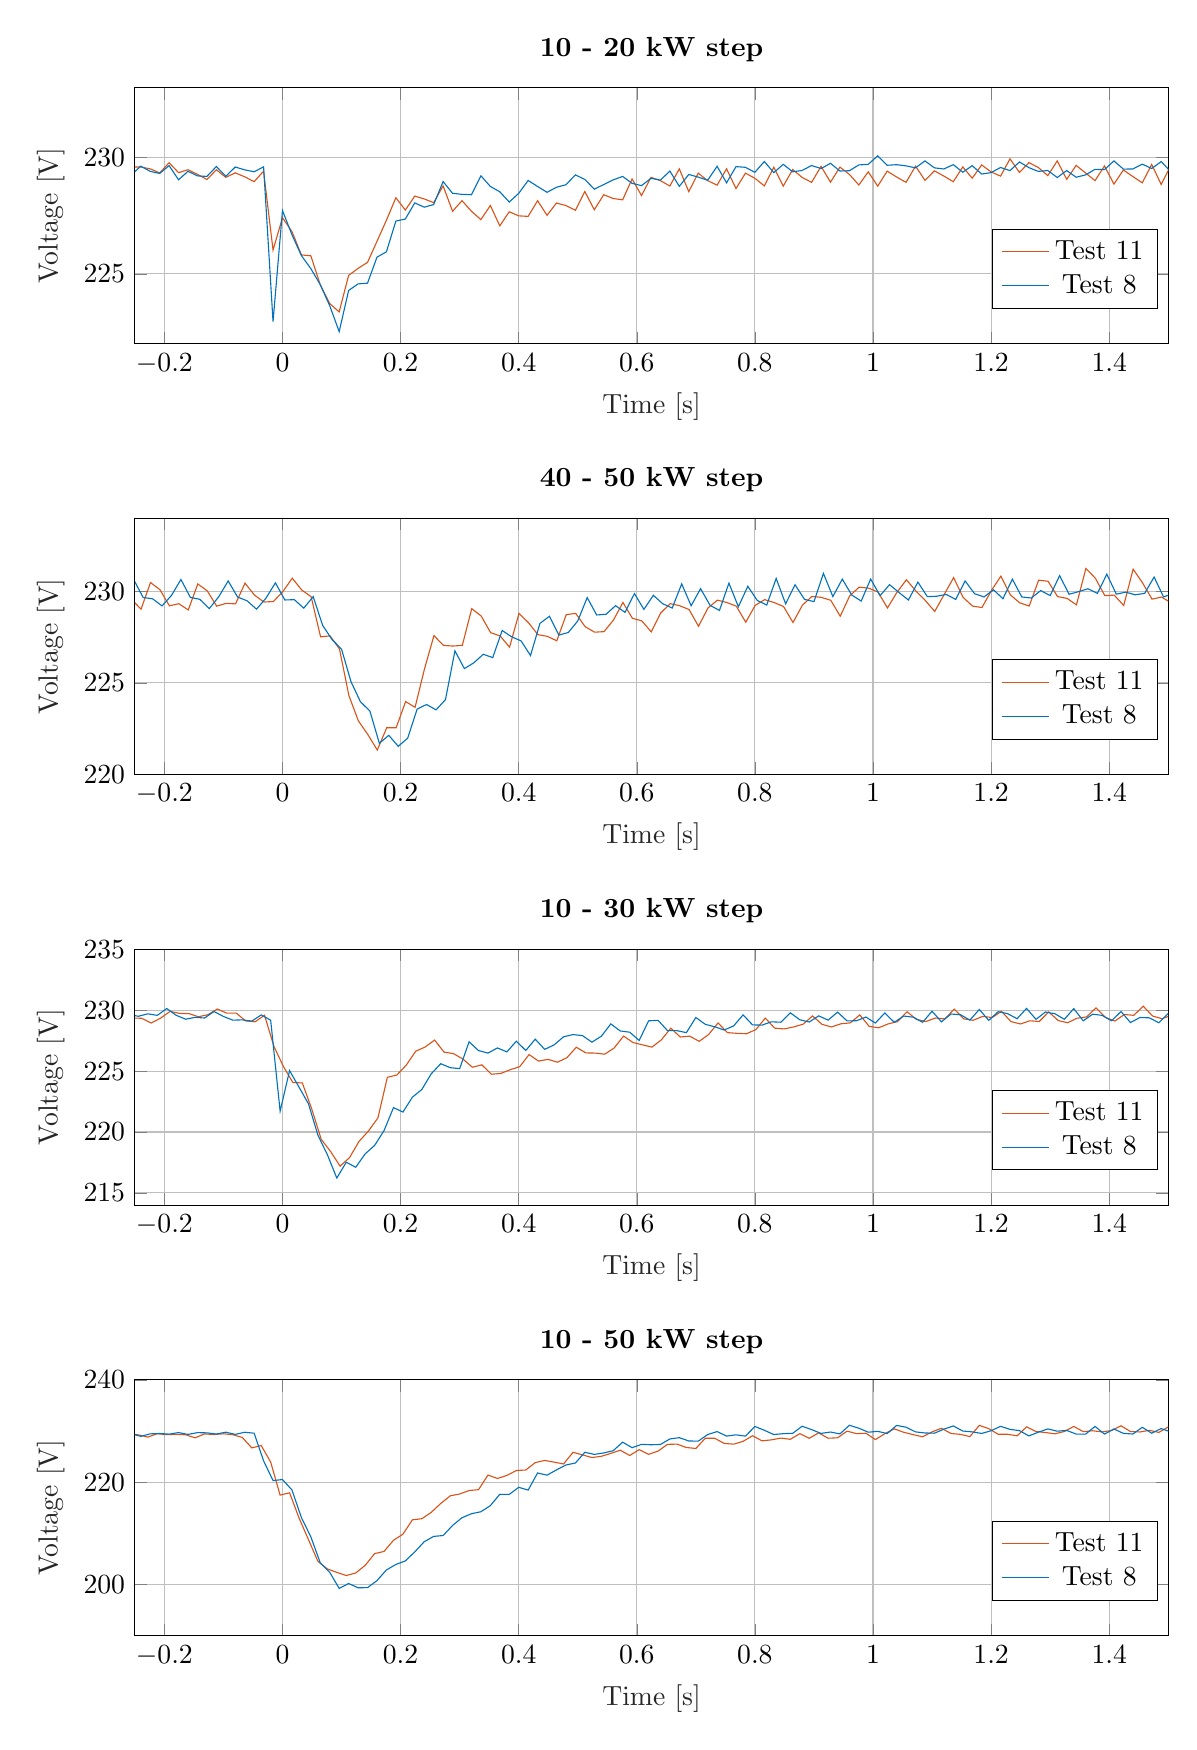
\begin{tikzpicture}

\begin{axis}[%
width=5.167in,
height=1.279in,
at={(0.867in,7.534in)},
scale only axis,
xmin=-0.25,
xmax=1.5,
xlabel style={font=\color{white!15!black}},
xlabel={Time [s]},
ymin=222,
ymax=233,
ylabel style={font=\color{white!15!black}},
ylabel={Voltage [V]},
axis background/.style={fill=white},
title style={font=\bfseries},
title={10 - 20 kW step},
%axis x line*=bottom,
%axis y line*=left
xmajorgrids,
ymajorgrids,
legend style={at={(0.99,0.45)},anchor=north east}
]
\addplot [color=mycolor1, solid]
  table[row sep=crcr]{%
-0.256	229.594893141072\\
-0.240000000000009	229.597533432729\\
-0.22399999999999	229.517203831768\\
-0.207999999999998	229.342181090907\\
-0.192000000000007	229.781191650706\\
-0.176000000000016	229.353286417014\\
-0.159999999999997	229.479194469117\\
-0.144000000000005	229.28309634014\\
-0.128000000000014	229.058862088113\\
-0.111999999999995	229.478401425993\\
-0.0960000000000036	229.153397223386\\
-0.0800000000000125	229.346375887397\\
-0.063999999999993	229.175680027837\\
-0.0480000000000018	228.968113996125\\
-0.0320000000000107	229.416358947826\\
-0.0159999999999911	226.026408539162\\
0	227.415292992161\\
0.0159999999999911	226.824147664588\\
0.0320000000000107	225.816560813206\\
0.0480000000000018	225.779475133607\\
0.063999999999993	224.525641695194\\
0.0800000000000125	223.7252180766\\
0.0960000000000036	223.364765085574\\
0.111999999999995	224.9372734363\\
0.128000000000014	225.238679165189\\
0.144000000000005	225.495491036295\\
0.175999999999988	227.307136185878\\
0.192000000000007	228.276023381396\\
0.207999999999998	227.744751566148\\
0.22399999999999	228.346498901479\\
0.240000000000009	228.224920230965\\
0.256	228.064081885726\\
0.271999999999991	228.785647018233\\
0.288000000000011	227.694699842239\\
0.304000000000002	228.147894361462\\
0.319999999999993	227.694393086729\\
0.336000000000013	227.335105295168\\
0.352000000000004	227.942006539794\\
0.367999999999995	227.067720874282\\
0.384000000000015	227.672460982196\\
0.400000000000006	227.496891694368\\
0.415999999999997	227.473447992058\\
0.431999999999988	228.14689285341\\
0.448000000000008	227.519873582955\\
0.463999999999999	228.048084625806\\
0.47999999999999	227.94019920417\\
0.496000000000009	227.737227778476\\
0.512	228.542490905319\\
0.527999999999992	227.758861820412\\
0.544000000000011	228.405565333313\\
0.560000000000002	228.242923217836\\
0.575999999999993	228.185045026892\\
0.592000000000013	229.083353633055\\
0.608000000000004	228.368387809511\\
0.623999999999995	229.152207806959\\
0.640000000000015	229.010277860129\\
0.656000000000006	228.779111918401\\
0.671999999999997	229.517131546111\\
0.687999999999988	228.538630684516\\
0.704000000000008	229.332063633026\\
0.719999999999999	229.011591300431\\
0.73599999999999	228.815345784449\\
0.75200000000001	229.520489479022\\
0.768000000000001	228.670050035168\\
0.783999999999992	229.333707787017\\
0.800000000000011	229.111497551335\\
0.816000000000003	228.78476431347\\
0.831999999999994	229.587496697356\\
0.848000000000013	228.774903571906\\
0.864000000000004	229.491292938616\\
0.879999999999995	229.148711642475\\
0.896000000000015	228.937313763522\\
0.912000000000006	229.626611500855\\
0.927999999999997	228.945757496032\\
0.943999999999988	229.591191395082\\
0.960000000000008	229.280629842641\\
0.975999999999999	228.823445460804\\
0.99199999999999	229.391024224914\\
1.00800000000001	228.77364935003\\
1.024	229.419899087393\\
1.03999999999999	229.166854050782\\
1.05600000000001	228.938921430183\\
1.072	229.634943752356\\
1.08799999999999	229.023172880483\\
1.10400000000001	229.432199732535\\
1.12	229.207367124736\\
1.136	228.965575036658\\
1.15200000000002	229.600154439647\\
1.16800000000001	229.11645732455\\
1.184	229.687356963109\\
1.19999999999999	229.384878990342\\
1.21600000000001	229.205681366804\\
1.232	229.948492325871\\
1.24799999999999	229.362070765008\\
1.26400000000001	229.786207080516\\
1.28	229.575148793284\\
1.29599999999999	229.226356922867\\
1.31200000000001	229.859792028346\\
1.328	229.066587264235\\
1.34399999999999	229.668113703591\\
1.376	229.010226227955\\
1.392	229.642617793009\\
1.40800000000002	228.8609704201\\
1.42400000000001	229.470263686495\\
1.44	229.18664028852\\
1.45599999999999	228.919096232312\\
1.47200000000001	229.705692419309\\
1.488	228.8472025303\\
1.50399999999999	229.642773111874\\
};
\addlegendentry{Test 11}

\addplot [color=mycolor2, solid]
  table[row sep=crcr]{%
-0.256	229.259034065655\\
-0.240000000000009	229.633664557694\\
-0.22399999999999	229.410466278477\\
-0.207999999999998	229.320376277629\\
-0.192000000000007	229.656627794122\\
-0.175999999999988	229.047379988031\\
-0.159999999999997	229.413341060431\\
-0.144000000000005	229.215095147076\\
-0.128000000000014	229.193362053371\\
-0.111999999999995	229.617002774202\\
-0.0960000000000036	229.197764611183\\
-0.0800000000000125	229.596344664625\\
-0.063999999999993	229.475804245851\\
-0.0480000000000018	229.391211353035\\
-0.0320000000000107	229.605324675344\\
-0.0159999999999911	222.947772817164\\
0	227.724009479168\\
0.0159999999999911	226.688114047742\\
0.0320000000000107	225.788274293474\\
0.0480000000000018	225.22795799241\\
0.063999999999993	224.538086593297\\
0.0800000000000125	223.631745354665\\
0.0960000000000036	222.519419171351\\
0.111999999999995	224.288439164994\\
0.128000000000014	224.570635868611\\
0.144000000000005	224.601547790095\\
0.159999999999997	225.719076936514\\
0.175999999999988	225.950982357793\\
0.192000000000007	227.273086249086\\
0.207999999999998	227.358468008874\\
0.22399999999999	228.05377214986\\
0.240000000000009	227.869386718192\\
0.256	227.983388011283\\
0.271999999999991	228.971409444748\\
0.288000000000011	228.466537252619\\
0.304000000000002	228.421633478975\\
0.319999999999993	228.405105547057\\
0.336000000000013	229.221100314441\\
0.352000000000004	228.760825869602\\
0.367999999999995	228.532696847045\\
0.383999999999986	228.090022424992\\
0.400000000000006	228.463376899668\\
0.415999999999997	229.018342404364\\
0.431999999999988	228.759899013698\\
0.448000000000008	228.509443801909\\
0.463999999999999	228.725843657976\\
0.47999999999999	228.834304108031\\
0.496000000000009	229.257753846356\\
0.512	229.063706554168\\
0.527999999999992	228.643485490637\\
0.560000000000002	229.04374567414\\
0.575999999999993	229.192320686901\\
0.592000000000013	228.895262954532\\
0.608000000000004	228.794609741371\\
0.623999999999995	229.111513022069\\
0.639999999999986	229.034101520775\\
0.656000000000006	229.420721670777\\
0.671999999999997	228.766136598018\\
0.687999999999988	229.275727071853\\
0.704000000000008	229.164062383815\\
0.719999999999999	229.028226167243\\
0.73599999999999	229.628097612003\\
0.75200000000001	228.915640051849\\
0.768000000000001	229.614763071499\\
0.783999999999992	229.582950272004\\
0.800000000000011	229.370278682605\\
0.816000000000003	229.834532589427\\
0.831999999999994	229.354844610515\\
0.848000000000013	229.711731772298\\
0.864000000000004	229.39070999571\\
0.879999999999995	229.449556565817\\
0.895999999999987	229.662014487451\\
0.912000000000006	229.530935945904\\
0.927999999999997	229.755691703703\\
0.943999999999988	229.424708576421\\
0.960000000000008	229.437684006142\\
0.975999999999999	229.686379524498\\
0.99199999999999	229.712631146526\\
1.00800000000001	230.079258905402\\
1.024	229.672015641485\\
1.03999999999999	229.696901553342\\
1.05600000000001	229.645777435992\\
1.072	229.560341540848\\
1.08799999999999	229.859435328326\\
1.10400000000001	229.55989778995\\
1.12	229.512689965262\\
1.136	229.698840715079\\
1.15199999999999	229.371954240125\\
1.16800000000001	229.654924984385\\
1.184	229.2947825531\\
1.19999999999999	229.356347948928\\
1.21600000000001	229.577444423169\\
1.232	229.442725901894\\
1.24799999999999	229.813756351569\\
1.26400000000001	229.569979919468\\
1.28	229.408801163032\\
1.29599999999999	229.447101175542\\
1.31200000000001	229.145527089646\\
1.328	229.443546184263\\
1.34399999999999	229.1574752057\\
1.36000000000001	229.258036890033\\
1.376	229.497220705871\\
1.392	229.483568806696\\
1.40799999999999	229.859586306746\\
1.42400000000001	229.506542493657\\
1.44	229.513041286626\\
1.45599999999999	229.720058906553\\
1.47200000000001	229.533129909852\\
1.488	229.829820100242\\
1.50399999999999	229.403163795558\\
};
\addlegendentry{Test 8}
\end{axis}

\begin{axis}[%
width=5.167in,
height=1.279in,
at={(0.867in,5.381in)},
scale only axis,
xmin=-0.25,
xmax=1.5,
xlabel style={font=\color{white!15!black}},
xlabel={Time [s]},
ymin=220,
ymax=234,
ylabel style={font=\color{white!15!black}},
ylabel={Voltage [V]},
axis background/.style={fill=white},
title style={font=\bfseries},
title={40 - 50 kW step},
%axis x line*=bottom,
%axis y line*=left
xmajorgrids,
ymajorgrids,
legend style={at={(0.99,0.45)},anchor=north east}
]
\addplot [color=mycolor1, solid]
  table[row sep=crcr]{%
-0.255500000000012	229.561408405763\\
-0.239500000000021	229.03785581884\\
-0.22350000000003	230.494315374119\\
-0.20750000000001	230.101585786784\\
-0.191500000000019	229.217474499314\\
-0.175500000000028	229.336502679851\\
-0.159500000000037	228.993534292762\\
-0.143500000000017	230.417175399674\\
-0.127500000000026	230.04156901302\\
-0.111500000000035	229.202518195008\\
-0.0955000000000155	229.354840677697\\
-0.0795000000000243	229.326780054588\\
-0.0635000000000332	230.458787654495\\
-0.0475000000000136	229.808597628894\\
-0.0315000000000225	229.427113046164\\
-0.0155000000000314	229.454579556395\\
0.000499999999988177	229.990076731959\\
0.0164999999999793	230.733374657206\\
0.0324999999999989	230.085912858541\\
0.04849999999999	229.720827593841\\
0.0644999999999811	227.520698714948\\
0.0805000000000007	227.575585532173\\
0.0964999999999918	226.857059326582\\
0.112499999999983	224.300474018765\\
0.128500000000003	222.920397330374\\
0.144499999999994	222.178171648306\\
0.160499999999985	221.327437451402\\
0.176500000000004	222.544267339288\\
0.192499999999995	222.548962099366\\
0.208499999999987	223.980231466105\\
0.224499999999978	223.663212819589\\
0.240499999999997	225.771384780395\\
0.256499999999988	227.589069227632\\
0.27249999999998	227.053901678286\\
0.288499999999999	227.017374081925\\
0.30449999999999	227.054556914651\\
0.320499999999981	229.063761827993\\
0.336500000000001	228.661012585298\\
0.352499999999992	227.748614559905\\
0.368499999999983	227.574508265602\\
0.384500000000003	226.955816665418\\
0.400499999999994	228.802965203106\\
0.416499999999985	228.297509918196\\
0.432500000000005	227.641663254172\\
0.448499999999996	227.548519088007\\
0.464499999999987	227.30437992081\\
0.480499999999978	228.737247513864\\
0.496499999999998	228.805369699677\\
0.512499999999989	228.079108648766\\
0.52849999999998	227.777257534125\\
0.544499999999999	227.806182266279\\
0.56049999999999	228.440993473323\\
0.576499999999982	229.404252371529\\
0.592500000000001	228.538522920094\\
0.608499999999992	228.395263624541\\
0.624499999999983	227.794191979496\\
0.640500000000003	228.825146801581\\
0.656499999999994	229.338519333367\\
0.672499999999985	229.226406372857\\
0.688500000000005	229.016822451359\\
0.704499999999996	228.102096537339\\
0.720499999999987	229.098492569916\\
0.736499999999978	229.530602732923\\
0.752499999999998	229.400761548726\\
0.768499999999989	229.199723723832\\
0.78449999999998	228.32109299858\\
0.8005	229.24466617878\\
0.816499999999991	229.558406646516\\
0.832499999999982	229.399339399684\\
0.848500000000001	229.181817539719\\
0.864499999999993	228.306958073323\\
0.880499999999984	229.257280046909\\
0.896500000000003	229.733742804175\\
0.912499999999994	229.683661126977\\
0.928499999999985	229.520841825595\\
0.944500000000005	228.650698906561\\
0.960499999999996	229.763934970744\\
0.976499999999987	230.240482412386\\
0.992499999999978	230.187739236141\\
1.0085	229.973569199184\\
1.02449999999999	229.101497898597\\
1.04049999999998	229.956212919068\\
1.0565	230.643114315917\\
1.07249999999999	230.037538999355\\
1.08849999999998	229.511750155766\\
1.1045	228.913356898716\\
1.13649999999998	230.764086061509\\
1.1525	229.683699352772\\
1.16849999999999	229.204283755213\\
1.18449999999999	229.125626757967\\
1.20050000000001	230.057966747538\\
1.2165	230.843586872558\\
1.23249999999999	229.820291014518\\
1.24849999999998	229.382623575772\\
1.2645	229.208581560346\\
1.28049999999999	230.624449718513\\
1.29649999999998	230.562368793749\\
1.3125	229.726080437389\\
1.32849999999999	229.626685527297\\
1.34449999999998	229.273872606493\\
1.3605	231.264923758306\\
1.37649999999999	230.731598494859\\
1.39249999999998	229.77741650822\\
1.4085	229.804373488513\\
1.42449999999999	229.237813632579\\
1.44049999999999	231.225571241671\\
1.45650000000001	230.474012968512\\
1.4725	229.584698174446\\
1.48849999999999	229.699901869042\\
1.50449999999998	229.39188548342\\
};
\addlegendentry{Test 11}

\addplot [color=mycolor2, solid]
  table[row sep=crcr]{%
-0.25200000000001	230.657161294545\\
-0.236000000000018	229.676077579585\\
-0.219999999999999	229.604519145093\\
-0.204000000000008	229.214052887828\\
-0.188000000000017	229.788124695872\\
-0.171999999999997	230.660675877931\\
-0.156000000000006	229.679216679488\\
-0.140000000000015	229.576084955171\\
-0.123999999999995	229.066190243604\\
-0.108000000000004	229.713818042475\\
-0.092000000000013	230.580372275807\\
-0.0759999999999934	229.701273828344\\
-0.0600000000000023	229.495895048248\\
-0.0440000000000111	229.036403827056\\
-0.0279999999999916	229.637823982224\\
-0.0120000000000005	230.478811857926\\
0.00399999999999068	229.539215778015\\
0.0200000000000102	229.557790416363\\
0.0360000000000014	229.089090106648\\
0.0519999999999925	229.725508041513\\
0.0680000000000121	228.145404594434\\
0.0840000000000032	227.371152330307\\
0.0999999999999943	226.850369040369\\
0.116000000000014	225.067260056974\\
0.132000000000005	223.969460856129\\
0.147999999999996	223.461404083249\\
0.164000000000016	221.699266485029\\
0.180000000000007	222.131570394474\\
0.195999999999998	221.530826099908\\
0.211999999999989	221.974286665762\\
0.228000000000009	223.568702949398\\
0.244	223.819907384035\\
0.259999999999991	223.523161500473\\
0.27600000000001	224.085725173237\\
0.292000000000002	226.756008260959\\
0.307999999999993	225.783312586139\\
0.324000000000012	226.100211841222\\
0.340000000000003	226.568356565034\\
0.355999999999995	226.385444461583\\
0.372000000000014	227.867735253133\\
0.388000000000005	227.524076886023\\
0.403999999999996	227.301463433923\\
0.420000000000016	226.498090893529\\
0.436000000000007	228.259296523205\\
0.451999999999998	228.646499768057\\
0.467999999999989	227.618236175859\\
0.484000000000009	227.759826442425\\
0.5	228.391244177568\\
0.515999999999991	229.671443016876\\
0.532000000000011	228.71908324782\\
0.548000000000002	228.758127040357\\
0.563999999999993	229.227832642985\\
0.580000000000013	228.861627154676\\
0.596000000000004	229.887350830736\\
0.611999999999995	229.023929878925\\
0.628000000000014	229.795685136493\\
0.644000000000005	229.33118494774\\
0.659999999999997	229.09859024179\\
0.676000000000016	230.418491386258\\
0.692000000000007	229.223790810989\\
0.707999999999998	230.158365041501\\
0.72399999999999	229.247936698356\\
0.740000000000009	228.96640471732\\
0.756	230.46316409959\\
0.771999999999991	229.169599832963\\
0.788000000000011	230.287782796537\\
0.804000000000002	229.5132729945\\
0.819999999999993	229.262262303371\\
0.836000000000013	230.718135437436\\
0.852000000000004	229.330288803874\\
0.867999999999995	230.372353530648\\
0.884000000000015	229.57082589941\\
0.900000000000006	229.450031842589\\
0.915999999999997	230.992507802526\\
0.932000000000016	229.728135735208\\
0.948000000000008	230.680071665386\\
0.963999999999999	229.808742431885\\
0.97999999999999	229.481185974456\\
0.996000000000009	230.683176108015\\
1.012	229.776887479283\\
1.02799999999999	230.377988366188\\
1.04400000000001	229.949136633382\\
1.06	229.538143098871\\
1.07599999999999	230.515476007127\\
1.09200000000001	229.722096121419\\
1.108	229.743854409472\\
1.124	229.842070558922\\
1.14000000000001	229.569977799717\\
1.15600000000001	230.580894916615\\
1.172	229.882361673683\\
1.18800000000002	229.705823301768\\
1.20400000000001	230.096546979126\\
1.22	229.609340151519\\
1.23599999999999	230.676442997835\\
1.25200000000001	229.704401024046\\
1.268	229.647048799177\\
1.28399999999999	230.053889011409\\
1.30000000000001	229.780108104251\\
1.316	230.87219186443\\
1.33199999999999	229.85321463451\\
1.34800000000001	229.994507238923\\
1.364	230.153481093022\\
1.38	229.902072460373\\
1.39600000000002	230.950176514592\\
1.41200000000001	229.857294790684\\
1.428	229.969607424457\\
1.44399999999999	229.822524975388\\
1.46000000000001	229.900858393728\\
1.476	230.793576168335\\
1.49199999999999	229.707585385976\\
1.50800000000001	229.889868297599\\
};
\addlegendentry{Test 8}
\end{axis}

\begin{axis}[%
width=5.167in,
height=1.279in,
at={(0.867in,3.227in)},
scale only axis,
xmin=-0.25,
xmax=1.5,
xlabel style={font=\color{white!15!black}},
xlabel={Time [s]},
ymin=214,
ymax=235,
ylabel style={font=\color{white!15!black}},
ylabel={Voltage [V]},
axis background/.style={fill=white},
title style={font=\bfseries},
title={10 - 30 kW step},
%axis x line*=bottom,
%axis y line*=left
xmajorgrids,
ymajorgrids,
legend style={at={(0.99,0.45)},anchor=north east}
]
\addplot [color=mycolor1, solid]
  table[row sep=crcr]{%
-0.254400000000032	229.360337078303\\
-0.238400000000041	229.335173477579\\
-0.222400000000022	228.942589314625\\
-0.206400000000031	229.34681711315\\
-0.190400000000039	229.898606581838\\
-0.17440000000002	229.739663959503\\
-0.158400000000029	229.716296892719\\
-0.142400000000038	229.460299708214\\
-0.126400000000018	229.62884199592\\
-0.110400000000027	230.096665525129\\
-0.0944000000000358	229.753259102104\\
-0.0784000000000162	229.761584424053\\
-0.0624000000000251	229.118604934431\\
-0.046400000000034	229.048369033875\\
-0.0304000000000144	229.582821760923\\
-0.0144000000000233	227.019681435151\\
0.00159999999999627	225.372564132742\\
0.0175999999999874	224.065265257178\\
0.0335999999999785	224.025919558114\\
0.0495999999999981	221.88015059127\\
0.0655999999999892	219.397138648559\\
0.0815999999999804	218.387241319027\\
0.0975999999999999	217.192985663592\\
0.113599999999991	217.900365133839\\
0.129599999999982	219.226083111155\\
0.145599999999973	220.081191937516\\
0.161599999999993	221.154192915387\\
0.177599999999984	224.488893042449\\
0.193599999999975	224.674156930744\\
0.209599999999995	225.488692842627\\
0.225599999999986	226.630263804574\\
0.241599999999977	226.974857248216\\
0.257599999999997	227.548224467057\\
0.273599999999988	226.554152544831\\
0.289599999999979	226.433638446234\\
0.305599999999998	225.985444012248\\
0.321599999999989	225.313686941987\\
0.337599999999981	225.513087691699\\
0.3536	224.742504566836\\
0.369599999999991	224.804319426376\\
0.385599999999982	225.111159105595\\
0.401599999999974	225.358120118292\\
0.417599999999993	226.355811653736\\
0.433599999999984	225.821538368511\\
0.449599999999975	225.963733234217\\
0.465599999999995	225.730586221159\\
0.481599999999986	226.097318048344\\
0.497599999999977	226.958674737863\\
0.513599999999997	226.49220567632\\
0.529599999999988	226.47809932569\\
0.545599999999979	226.387808906801\\
0.561599999999999	226.89106664478\\
0.57759999999999	227.875719395223\\
0.593599999999981	227.341915892797\\
0.6096	227.156182184363\\
0.625599999999992	226.964712198725\\
0.641599999999983	227.563998231008\\
0.657599999999974	228.522071979197\\
0.673599999999993	227.798576096055\\
0.689599999999984	227.868475658701\\
0.705599999999976	227.443403764351\\
0.721599999999995	228.001935261364\\
0.737599999999986	228.950230390356\\
0.753599999999977	228.155865796581\\
0.769599999999997	228.099763966941\\
0.785599999999988	228.064572197434\\
0.801599999999979	228.404584151029\\
0.817599999999999	229.350185257305\\
0.83359999999999	228.523829396018\\
0.849599999999981	228.461349519466\\
0.865600000000001	228.624776349257\\
0.881599999999992	228.848994478167\\
0.897599999999983	229.524630393854\\
0.913599999999974	228.838974708453\\
0.929599999999994	228.621266994052\\
0.945599999999985	228.882196269249\\
0.961599999999976	228.95846341897\\
0.977599999999995	229.609803367428\\
0.993599999999986	228.66841045154\\
1.00959999999998	228.554921664773\\
1.0256	228.872240334353\\
1.04159999999999	229.060216343374\\
1.05759999999998	229.86794709192\\
1.0736	229.24406717228\\
1.08959999999999	229.069528311643\\
1.10559999999998	229.354378388433\\
1.1216	229.282818642101\\
1.13759999999999	230.086996956401\\
1.15359999999998	229.288519766675\\
1.16959999999997	229.168742693181\\
1.18559999999999	229.490715136958\\
1.20159999999998	229.396012464101\\
1.21759999999998	229.905663579334\\
1.2336	229.064676157527\\
1.24959999999999	228.869092416391\\
1.26559999999998	229.128319727856\\
1.2816	229.074369096373\\
1.29759999999999	229.854589479045\\
1.31359999999998	229.147175030013\\
1.3296	228.968637688259\\
1.34559999999999	229.341447867492\\
1.36159999999998	229.444767163211\\
1.37759999999997	230.191172312973\\
1.39359999999999	229.402812038102\\
1.40959999999998	229.107829403505\\
1.42559999999997	229.647173046845\\
1.44159999999999	229.577324074177\\
1.45759999999999	230.326318027668\\
1.47359999999998	229.515158134079\\
1.4896	229.29690193065\\
1.50559999999999	229.605194653778\\
};
\addlegendentry{Test 11}

\addplot [color=mycolor2, solid]
  table[row sep=crcr]{%
-0.260000000000019	229.642512728361\\
-0.244000000000028	229.498868246285\\
-0.228000000000009	229.702588597543\\
-0.212000000000018	229.574619936048\\
-0.196000000000026	230.136854075852\\
-0.180000000000007	229.579989937926\\
-0.164000000000016	229.258147846907\\
-0.148000000000025	229.413127527778\\
-0.132000000000005	229.356185773331\\
-0.116000000000014	229.892265760718\\
-0.100000000000023	229.482946288382\\
-0.0840000000000032	229.180526443337\\
-0.0680000000000121	229.204926425921\\
-0.0520000000000209	229.102727549518\\
-0.0360000000000298	229.610307802559\\
-0.0200000000000102	229.174935671793\\
-0.0040000000000191	221.709055121235\\
0.0120000000000005	225.042889654615\\
0.0439999999999827	222.312337966928\\
0.0600000000000023	219.737111301504\\
0.0759999999999934	218.135832728703\\
0.0919999999999845	216.219990029645\\
0.108000000000004	217.518725289499\\
0.123999999999995	217.104328673835\\
0.139999999999986	218.205217912633\\
0.155999999999977	218.895717878678\\
0.171999999999997	220.115682840976\\
0.187999999999988	222.002437079772\\
0.203999999999979	221.634098080408\\
0.219999999999999	222.858354647522\\
0.23599999999999	223.491272371455\\
0.251999999999981	224.782820376149\\
0.268000000000001	225.605509712803\\
0.283999999999992	225.280724417904\\
0.299999999999983	225.198981467051\\
0.316000000000003	227.400989720526\\
0.331999999999994	226.685114916778\\
0.347999999999985	226.477754005055\\
0.364000000000004	226.90086030033\\
0.379999999999995	226.577219901382\\
0.395999999999987	227.451319611723\\
0.411999999999978	226.690721137574\\
0.427999999999997	227.61871936839\\
0.443999999999988	226.783061361905\\
0.45999999999998	227.150724816589\\
0.475999999999999	227.817501689076\\
0.49199999999999	227.997178120578\\
0.507999999999981	227.910721302698\\
0.524000000000001	227.373401552932\\
0.539999999999992	227.862224821798\\
0.555999999999983	228.873671817738\\
0.572000000000003	228.293683374237\\
0.587999999999994	228.19198431806\\
0.603999999999985	227.514215751999\\
0.620000000000005	229.126832674173\\
0.635999999999996	229.165362868006\\
0.651999999999987	228.323425124451\\
0.667999999999978	228.316990491593\\
0.683999999999998	228.155343288027\\
0.699999999999989	229.399969348535\\
0.71599999999998	228.83878989871\\
0.731999999999999	228.634165775055\\
0.74799999999999	228.372885168603\\
0.763999999999982	228.708744859072\\
0.780000000000001	229.613564180708\\
0.795999999999992	228.793146218121\\
0.811999999999983	228.774100602073\\
0.828000000000003	229.044310766135\\
0.843999999999994	229.011423352536\\
0.859999999999985	229.780603415159\\
0.875999999999976	229.2130159682\\
0.891999999999996	229.026417903691\\
0.907999999999987	229.534066284656\\
0.923999999999978	229.184342353975\\
0.939999999999998	229.841213549734\\
0.955999999999989	229.118906092006\\
0.97199999999998	229.134568453853\\
0.988	229.433616132365\\
1.00399999999999	228.946847382733\\
1.01999999999998	229.7714533255\\
1.036	229.007050397077\\
1.05199999999999	229.516493338042\\
1.06799999999998	229.42651516427\\
1.084	229.003623676831\\
1.09999999999999	229.911117219095\\
1.11599999999999	229.045036227191\\
1.13199999999998	229.682739678841\\
1.148	229.632459038019\\
1.16399999999999	229.182671788473\\
1.17999999999998	230.057249496333\\
1.196	229.161428376955\\
1.21199999999999	229.878865653294\\
1.22799999999998	229.711675476866\\
1.244	229.29938053865\\
1.25999999999999	230.147404700738\\
1.27599999999998	229.24501901992\\
1.29199999999997	229.850749783567\\
1.30799999999999	229.707689950738\\
1.32399999999998	229.251633480232\\
1.33999999999998	230.127085410466\\
1.35599999999999	229.129455422576\\
1.37199999999999	229.670498082441\\
1.38799999999998	229.575415343853\\
1.404	229.128742266934\\
1.41999999999999	229.889241479371\\
1.43599999999998	228.984460195173\\
1.45199999999997	229.398301418887\\
1.46799999999999	229.372782124806\\
1.48399999999998	228.964554911992\\
1.49999999999997	229.742044834757\\
1.51599999999999	229.1628518817\\
};
\addlegendentry{Test 8}
\end{axis}

\begin{axis}[%
width=5.167in,
height=1.279in,
at={(0.867in,1.074in)},
scale only axis,
xmin=-0.25,
xmax=1.5,
xlabel style={font=\color{white!15!black}},
xlabel={Time [s]},
ymin=190,
ymax=240,
ylabel style={font=\color{white!15!black}},
ylabel={Voltage [V]},
axis background/.style={fill=white},
title style={font=\bfseries},
title={10 - 50 kW step},
%axis x line*=bottom,
%axis y line*=left
xmajorgrids,
ymajorgrids,
legend style={at={(0.99,0.45)},anchor=north east}
]
\addplot [color=mycolor1, solid]
  table[row sep=crcr]{%
-0.260000000000019	229.513015200559\\
-0.244000000000028	229.258684371694\\
-0.228000000000037	228.819045015631\\
-0.212000000000018	229.476230673908\\
-0.196000000000026	229.287233608959\\
-0.180000000000035	229.354808923975\\
-0.164000000000044	229.265425012151\\
-0.148000000000025	228.679377796388\\
-0.132000000000033	229.44124859342\\
-0.116000000000042	229.316438918283\\
-0.100000000000023	229.464875659363\\
-0.0840000000000316	229.278211643587\\
-0.0680000000000405	228.741545376781\\
-0.0520000000000209	226.70243636262\\
-0.0360000000000298	227.166338342628\\
-0.0200000000000387	223.940473065044\\
-0.00400000000004752	217.470217842924\\
0.011999999999972	217.937500285017\\
0.0279999999999632	213.01763762149\\
0.0599999999999739	204.526217500835\\
0.075999999999965	203.047232418536\\
0.0919999999999561	202.371596161495\\
0.107999999999976	201.760336451302\\
0.123999999999967	202.250484152177\\
0.139999999999958	203.744334980633\\
0.155999999999977	206.041863404798\\
0.171999999999969	206.464723287532\\
0.18799999999996	208.651158027736\\
0.203999999999979	209.838539667461\\
0.21999999999997	212.643661920269\\
0.235999999999962	212.86304746088\\
0.251999999999981	214.11789158097\\
0.267999999999972	215.842652394795\\
0.283999999999963	217.328301527235\\
0.299999999999983	217.696224223078\\
0.315999999999974	218.368058119048\\
0.331999999999965	218.541351211241\\
0.347999999999956	221.395023883048\\
0.363999999999976	220.724668595315\\
0.379999999999967	221.322520768242\\
0.395999999999958	222.284256278637\\
0.411999999999978	222.382150750261\\
0.427999999999969	223.828163479882\\
0.44399999999996	224.255063153371\\
0.45999999999998	223.920004361153\\
0.475999999999971	223.566927592883\\
0.491999999999962	225.84463258074\\
0.507999999999953	225.34007931539\\
0.523999999999972	224.819999876613\\
0.539999999999964	225.063741701548\\
0.555999999999955	225.63387873904\\
0.571999999999974	226.254976389959\\
0.587999999999965	225.221981467491\\
0.603999999999957	226.360555169345\\
0.619999999999976	225.451378159069\\
0.635999999999967	226.082646527269\\
0.651999999999958	227.396646883556\\
0.667999999999978	227.445037959479\\
0.683999999999969	226.780586056189\\
0.69999999999996	226.594197463781\\
0.71599999999998	228.593844541134\\
0.731999999999971	228.580304257027\\
0.747999999999962	227.586409493891\\
0.763999999999982	227.43435254597\\
0.779999999999973	227.981663546598\\
0.795999999999964	229.080553981738\\
0.811999999999983	228.085548391339\\
0.827999999999975	228.275057985379\\
0.843999999999966	228.622895906687\\
0.859999999999957	228.382461409945\\
0.875999999999976	229.49132042219\\
0.891999999999967	228.588054484666\\
0.907999999999959	229.640390084592\\
0.923999999999978	228.598269668978\\
0.939999999999969	228.673368903114\\
0.95599999999996	229.981565670133\\
0.97199999999998	229.499242305525\\
0.987999999999971	229.563787181686\\
1.00399999999996	228.335612013469\\
1.01999999999995	229.479249793592\\
1.03599999999997	230.430394065677\\
1.05199999999996	229.757245802113\\
1.06799999999996	229.297837526702\\
1.08399999999997	228.870446565338\\
1.09999999999997	229.842356020379\\
1.11599999999996	230.543973502399\\
1.13199999999998	229.522782057988\\
1.14799999999997	229.351485930536\\
1.16399999999996	228.912979693686\\
1.17999999999998	231.102685228418\\
1.19599999999997	230.469563985605\\
1.21199999999996	229.368842583985\\
1.22799999999998	229.371747623747\\
1.24399999999997	229.063857193156\\
1.25999999999996	230.817762457846\\
1.27599999999998	229.910908581616\\
1.29199999999997	229.709220421805\\
1.30799999999996	229.460174557477\\
1.32399999999998	229.903512510622\\
1.33999999999998	230.905339631105\\
1.35599999999997	229.880606556472\\
1.37199999999996	230.055053884116\\
1.38799999999998	229.825341127838\\
1.40399999999997	230.10937849483\\
1.41999999999996	231.033750554885\\
1.43599999999998	229.900498752279\\
1.45199999999997	229.817730848726\\
1.46799999999996	230.143319550204\\
1.48399999999998	229.733608745715\\
1.49999999999997	230.799716258267\\
1.51599999999996	229.982458462769\\
};
\addlegendentry{Test 11}

\addplot [color=mycolor2, solid]
  table[row sep=crcr]{%
-0.256000000000029	229.452881358327\\
-0.240000000000038	228.968342398354\\
-0.224000000000018	229.450565800706\\
-0.208000000000027	229.520700264437\\
-0.192000000000036	229.396824364227\\
-0.176000000000016	229.697588662013\\
-0.160000000000025	229.342446225986\\
-0.144000000000034	229.687603871069\\
-0.128000000000014	229.648963970161\\
-0.112000000000023	229.417109656277\\
-0.0960000000000321	229.775048662789\\
-0.0800000000000125	229.346572272139\\
-0.0640000000000214	229.759771788246\\
-0.0480000000000302	229.579489894458\\
-0.0320000000000391	224.166683275968\\
-0.0160000000000196	220.323078042144\\
-2.8421709430404e-14	220.51488807548\\
0.0159999999999911	218.48859294015\\
0.0319999999999823	213.097056926378\\
0.0480000000000018	209.326250079888\\
0.063999999999993	204.23394924644\\
0.0799999999999841	202.387616443055\\
0.0960000000000036	199.236538671744\\
0.111999999999995	200.197086581226\\
0.127999999999986	199.360223093882\\
0.144000000000005	199.393968827004\\
0.159999999999997	200.755066487199\\
0.175999999999988	202.845008119863\\
0.191999999999979	203.922817418315\\
0.207999999999998	204.610064217666\\
0.22399999999999	206.381584972091\\
0.239999999999981	208.366334458204\\
0.256	209.405680095814\\
0.271999999999991	209.573219125046\\
0.287999999999982	211.538918643058\\
0.304000000000002	213.057416510617\\
0.319999999999993	213.841368232295\\
0.335999999999984	214.220410909275\\
0.352000000000004	215.420471962649\\
0.367999999999995	217.635222316228\\
0.383999999999986	217.610849862975\\
0.399999999999977	218.99947324587\\
0.415999999999997	218.456108818699\\
0.431999999999988	221.80051097794\\
0.447999999999979	221.375582741985\\
0.463999999999999	222.40236730584\\
0.47999999999999	223.3610991746\\
0.495999999999981	223.74865889665\\
0.512	225.845535692629\\
0.527999999999992	225.432811742824\\
0.543999999999983	225.718600525298\\
0.560000000000002	226.153342379993\\
0.575999999999993	227.822907559961\\
0.591999999999985	226.751880994861\\
0.608000000000004	227.392037876646\\
0.623999999999995	227.320494139324\\
0.639999999999986	227.375033546624\\
0.655999999999977	228.456796489274\\
0.671999999999997	228.701598887519\\
0.687999999999988	228.062682537166\\
0.703999999999979	228.017059160967\\
0.719999999999999	229.317319154584\\
0.73599999999999	229.897751313276\\
0.751999999999981	229.017707383381\\
0.768000000000001	229.260238715856\\
0.783999999999992	229.007378834563\\
0.799999999999983	230.88631343687\\
0.816000000000003	230.152355869361\\
0.831999999999994	229.312388332828\\
0.847999999999985	229.487458914991\\
0.864000000000004	229.560333976115\\
0.879999999999995	230.940951910252\\
0.895999999999987	230.275903182037\\
0.911999999999978	229.53504801812\\
0.927999999999997	229.807115784903\\
0.943999999999988	229.442907417126\\
0.95999999999998	231.126139595811\\
0.975999999999999	230.556559377302\\
0.99199999999999	229.77159684046\\
1.00799999999998	229.946252628044\\
1.024	229.498929173621\\
1.03999999999999	231.097202348574\\
1.05599999999998	230.752574673764\\
1.072	229.835511045872\\
1.08799999999999	229.621391218738\\
1.10399999999999	229.577933725082\\
1.12	230.361899109622\\
1.136	230.996097042733\\
1.15199999999999	230.002656532987\\
1.16799999999998	229.835385346012\\
1.184	229.526888388817\\
1.19999999999999	230.066657994349\\
1.21599999999998	230.920500268308\\
1.232	230.330564245024\\
1.24799999999999	230.075391148365\\
1.26399999999998	229.047961555549\\
1.28	229.772196165414\\
1.29599999999999	230.413688202068\\
1.31199999999998	229.975050472752\\
1.328	230.120319997252\\
1.34399999999999	229.410967305444\\
1.35999999999999	229.397806383957\\
1.376	230.903698875236\\
1.392	229.406708330034\\
1.40799999999999	230.404927461002\\
1.42399999999998	229.543076425023\\
1.44	229.418213861341\\
1.45599999999999	230.727655098938\\
1.47199999999998	229.573485806519\\
1.488	230.486760115983\\
1.50399999999999	229.832110062916\\
};
\addlegendentry{Test 8}
\end{axis}
\end{tikzpicture}%
\caption{Voltage disturbance due to various changes in load without and with controller.}
\label{fig:test8+11volt-1020-4050-1030-1050}
\end{figure}

First thing that appears when applying the controller is that the Voltage disturbance is corrected a bit faster than without controller. The other thing is that at lower loads a small drop appears in the 10 to 20 kW and 10 to 30 kW steps visible at the 0.4 second mark. While the 40 to 50 kW steps experiencing a larger and longer lasting overshoot does not give the drop in voltage. Contrary to the frequency no visible improvement is attained in the steady state time by applying the designed controller.
The reason for this could be that the governor and the AVR functions as two independent systems.  


%From the voltage measurements it can be concluded that the response of the controlled signal has the same characteristic as the characteristic of the simulated controller in the \secref{system_design_implementation} \figref{fig:dist_out} which is expected. From the frequency measurements it can be seen that the controller affects the system which makes it faster to respond on load changes. For big load steps as shown in \figref{fig:test8+11freq-1050-1030-4050} the controller was slower than it was on the other measurements. It has not been analyzed any further how this test could be improved. To improved the controller the poles of the state feedback could be altered to see if it would have done any changes in the response of the controlled system.    


